
\section{Validation and Results}
\subsection{Validation}
% % % % % \begin{frame}{Validation of software}
% % % % %   
% % % % % % % % % % % % %   {\color{red}{METER ALGO SOBRE COMO SE CALCULAN LAS ENERGIAS PARA ATOMOS Y OSCILADORES HARMONICOS. EXPERIMENTAL SET UP?}}
% % % % %   \begin{scriptsize}
% % % % %     \begin{table}
% % % % %     \centering
% % % % %       \begin{tabular}{lcc}
% % % % %       \toprule[1pt]
% % % % %       \textbf{System} & $E_0$ (au) & $\alpha_{optimal}$ \\
% % % % %       \midrule[1pt]
% % % % %       He      &  4.0  &   2.0 \\
% % % % %       Be      & 20.0  &   4.0 \\
% % % % %       2DHO2e ($\omega=1.0$) & 1.0   &   1.0 \\
% % % % %       2DHO6e ($\omega = 1.0$) &  10.0  &  1.0  \\
% % % % %       \bottomrule[1pt]
% % % % %       \end{tabular}\caption{Analytical values of the ground state energy and corresponding variational parameter $\alpha$ computed for the Slater determinant. 2DHO2e (two-dimensional harmonic oscillator with two electrons). Set up: $dt=0.01$.}
% % % % %     \label{analyticalEnergyvsAlpha}
% % % % %     \end{table}
% % % % %   \end{scriptsize}
% % % % %   
% % % % % % % % % % % % %     \begin{scriptsize}
% % % % % % % % % % % % %     \begin{alertblock}{$E_{min}$ and $\alpha_{opt}$ without correlation}
% % % % % % % % % % % % %       \begin{table}
% % % % % % % % % % % % %       \centering
% % % % % % % % % % % % %         \begin{tabular}{lccc}
% % % % % % % % % % % % %           \toprule[1pt]
% % % % % % % % % % % % %           \textbf{System} & \textbf{dt} & \textbf{Monte Carlo cycles} & \textbf{Equilibration cycles} \\
% % % % % % % % % % % % %           \midrule[1pt]
% % % % % % % % % % % % %           He                      &  0.01   &   $1\times10^7$ & 10 \% \\
% % % % % % % % % % % % %           Be                      &  0.01   &   $1\times10^7$ & 10 \% \\
% % % % % % % % % % % % %           2DHO2e ($\omega=1.0$)   &  0.01   &   $1\times10^7$ & 10 \% \\
% % % % % % % % % % % % %           2DHO6e ($\omega = 1.0$) &  0.01   &   $1\times10^7$ & 10 \% \\
% % % % % % % % % % % % %           \bottomrule[1pt]
% % % % % % % % % % % % %         \end{tabular}\caption{Experimental setup used to compute the dependence of the energy on the variational parameter $\alpha$ when no correlation and Coulomb interation are included. All runs were carried out on one computer, that is only the serial version of the code was used.}
% % % % % % % % % % % % %         \label{expSetUpAlpha}
% % % % % % % % % % % % %     \end{table}
% % % % % % % % % % % % %     \end{alertblock}
% % % % % % % % % % % % %     \end{scriptsize}
% % % % %  \end{frame}
  


\begin{frame}{Analytical GS for atoms (without correlation)}
  \begin{figure}
  \begin{center}
    \begin{tabular}{cc}
      \resizebox{50mm}{!}{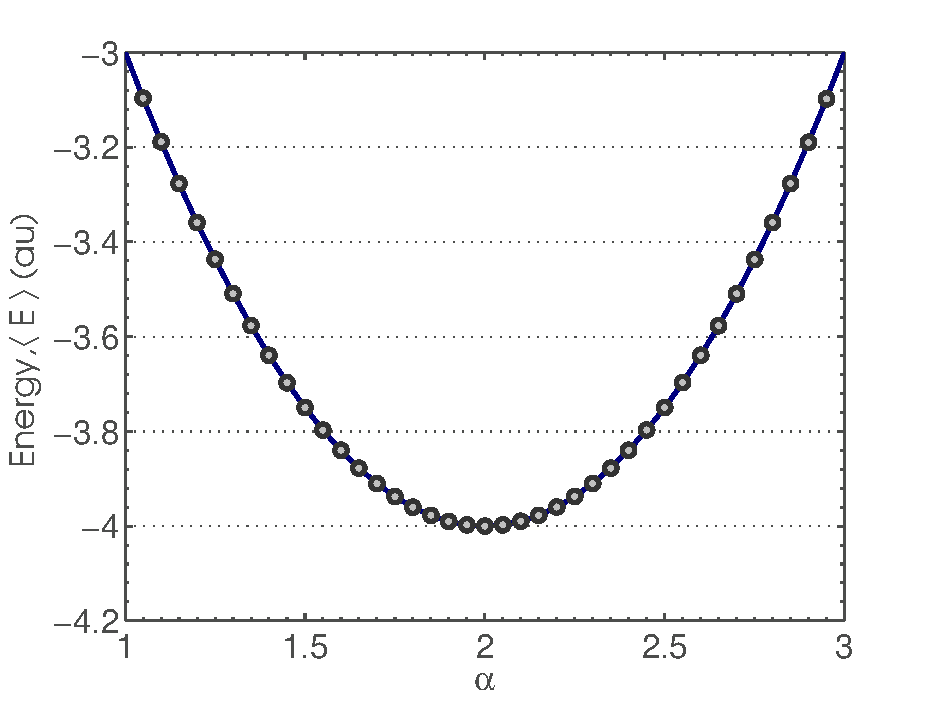
\includegraphics{figures/experimentalData/secondPart/alphaStudy/alphaHe}} &
      \resizebox{50mm}{!}{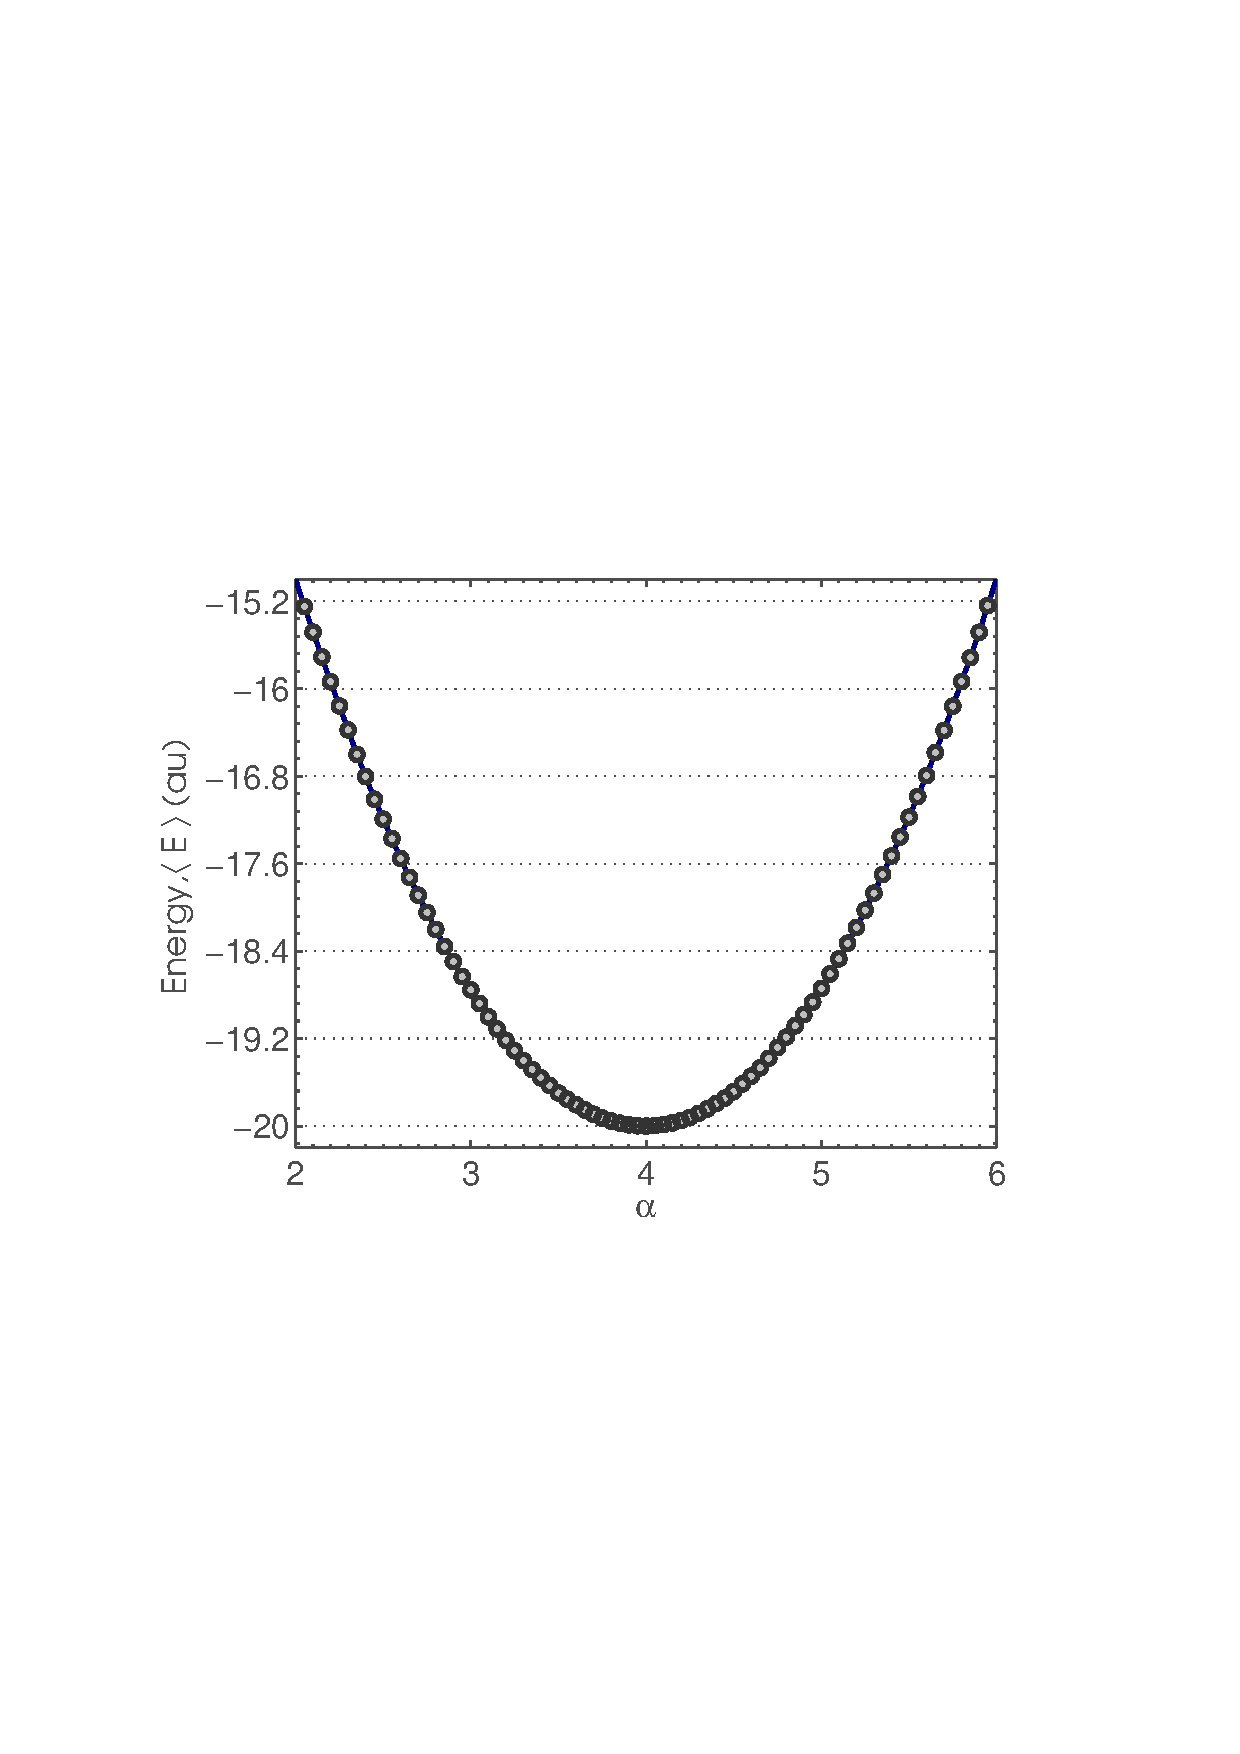
\includegraphics{figures/experimentalData/secondPart/alphaStudy/alphaBe}} \\
% % %        \resizebox{45mm}{!}{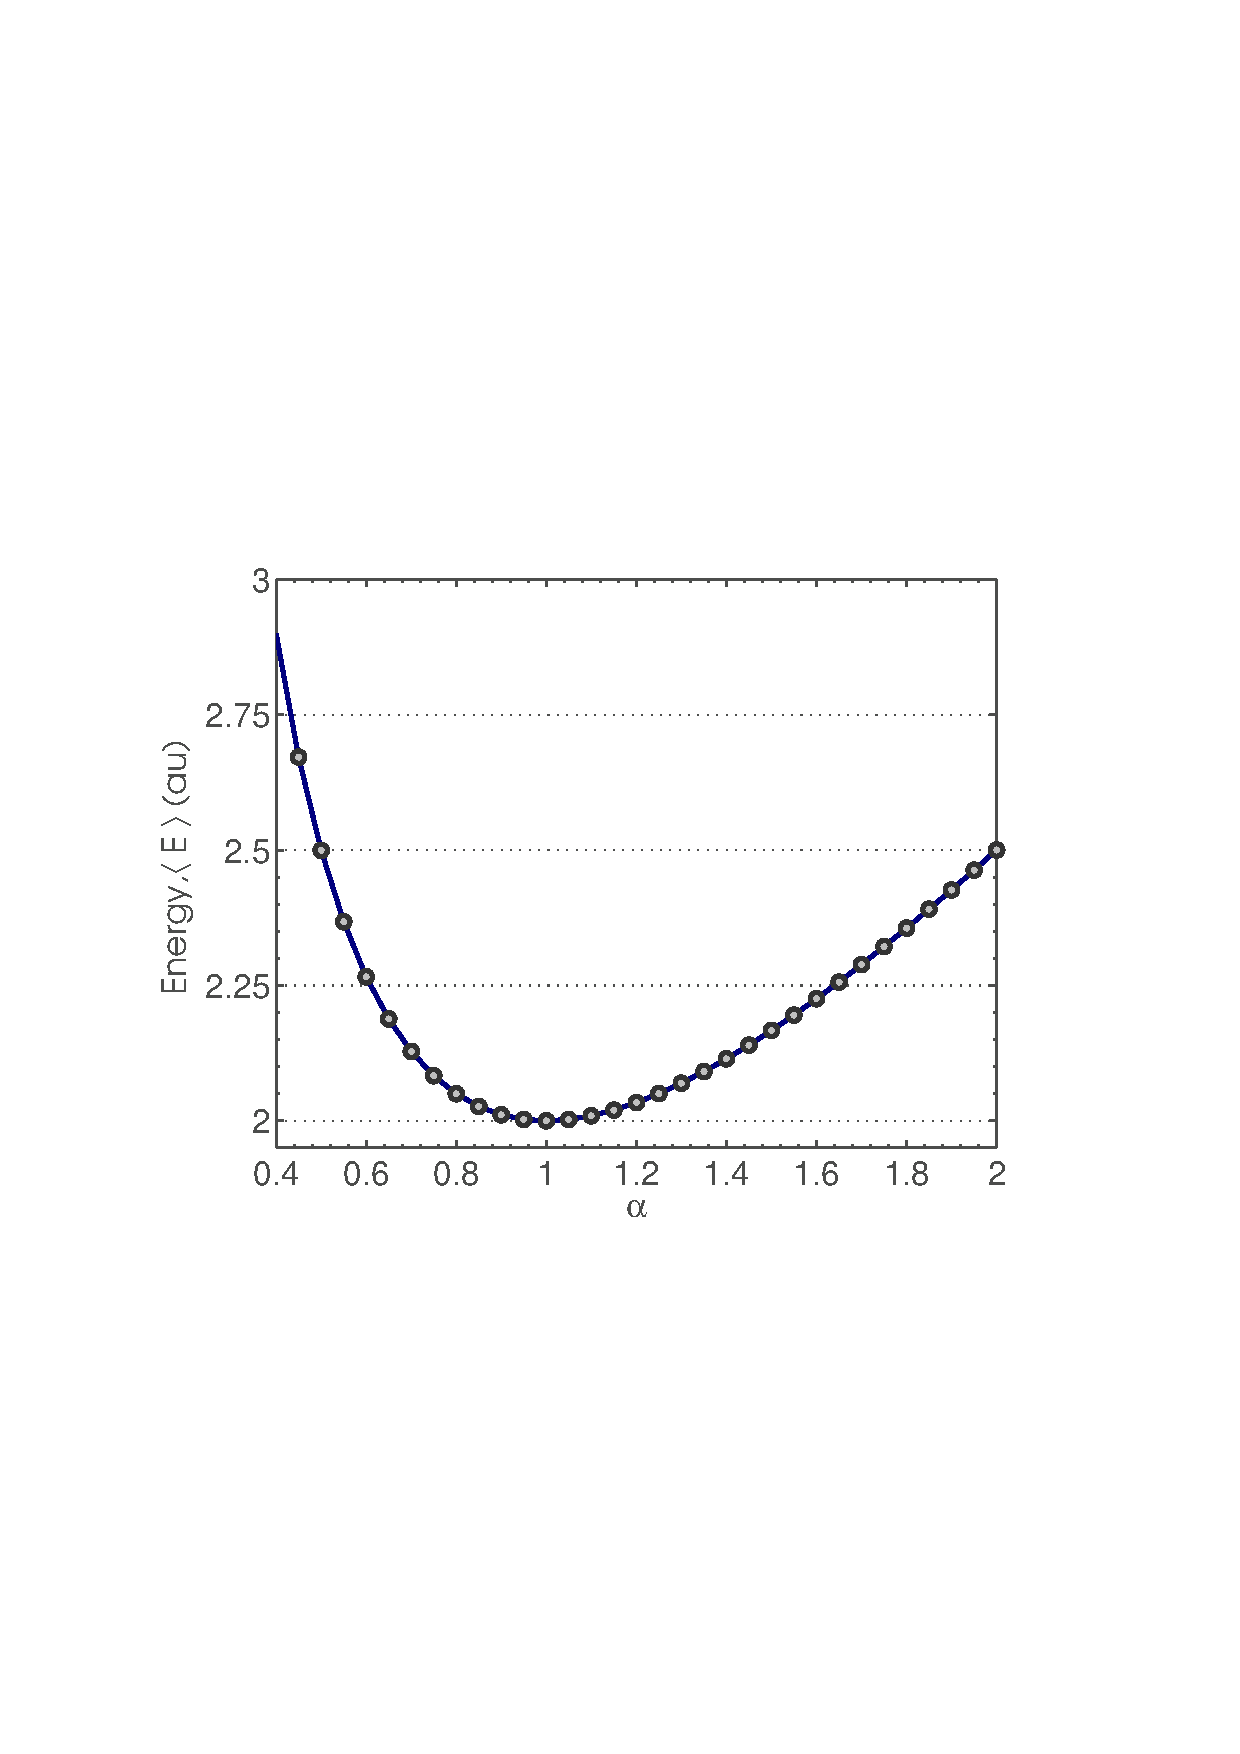
\includegraphics{figures/experimentalData/secondPart/alphaStudy/alpha2DHO2e}} &
% % %       \resizebox{75mm}{!}{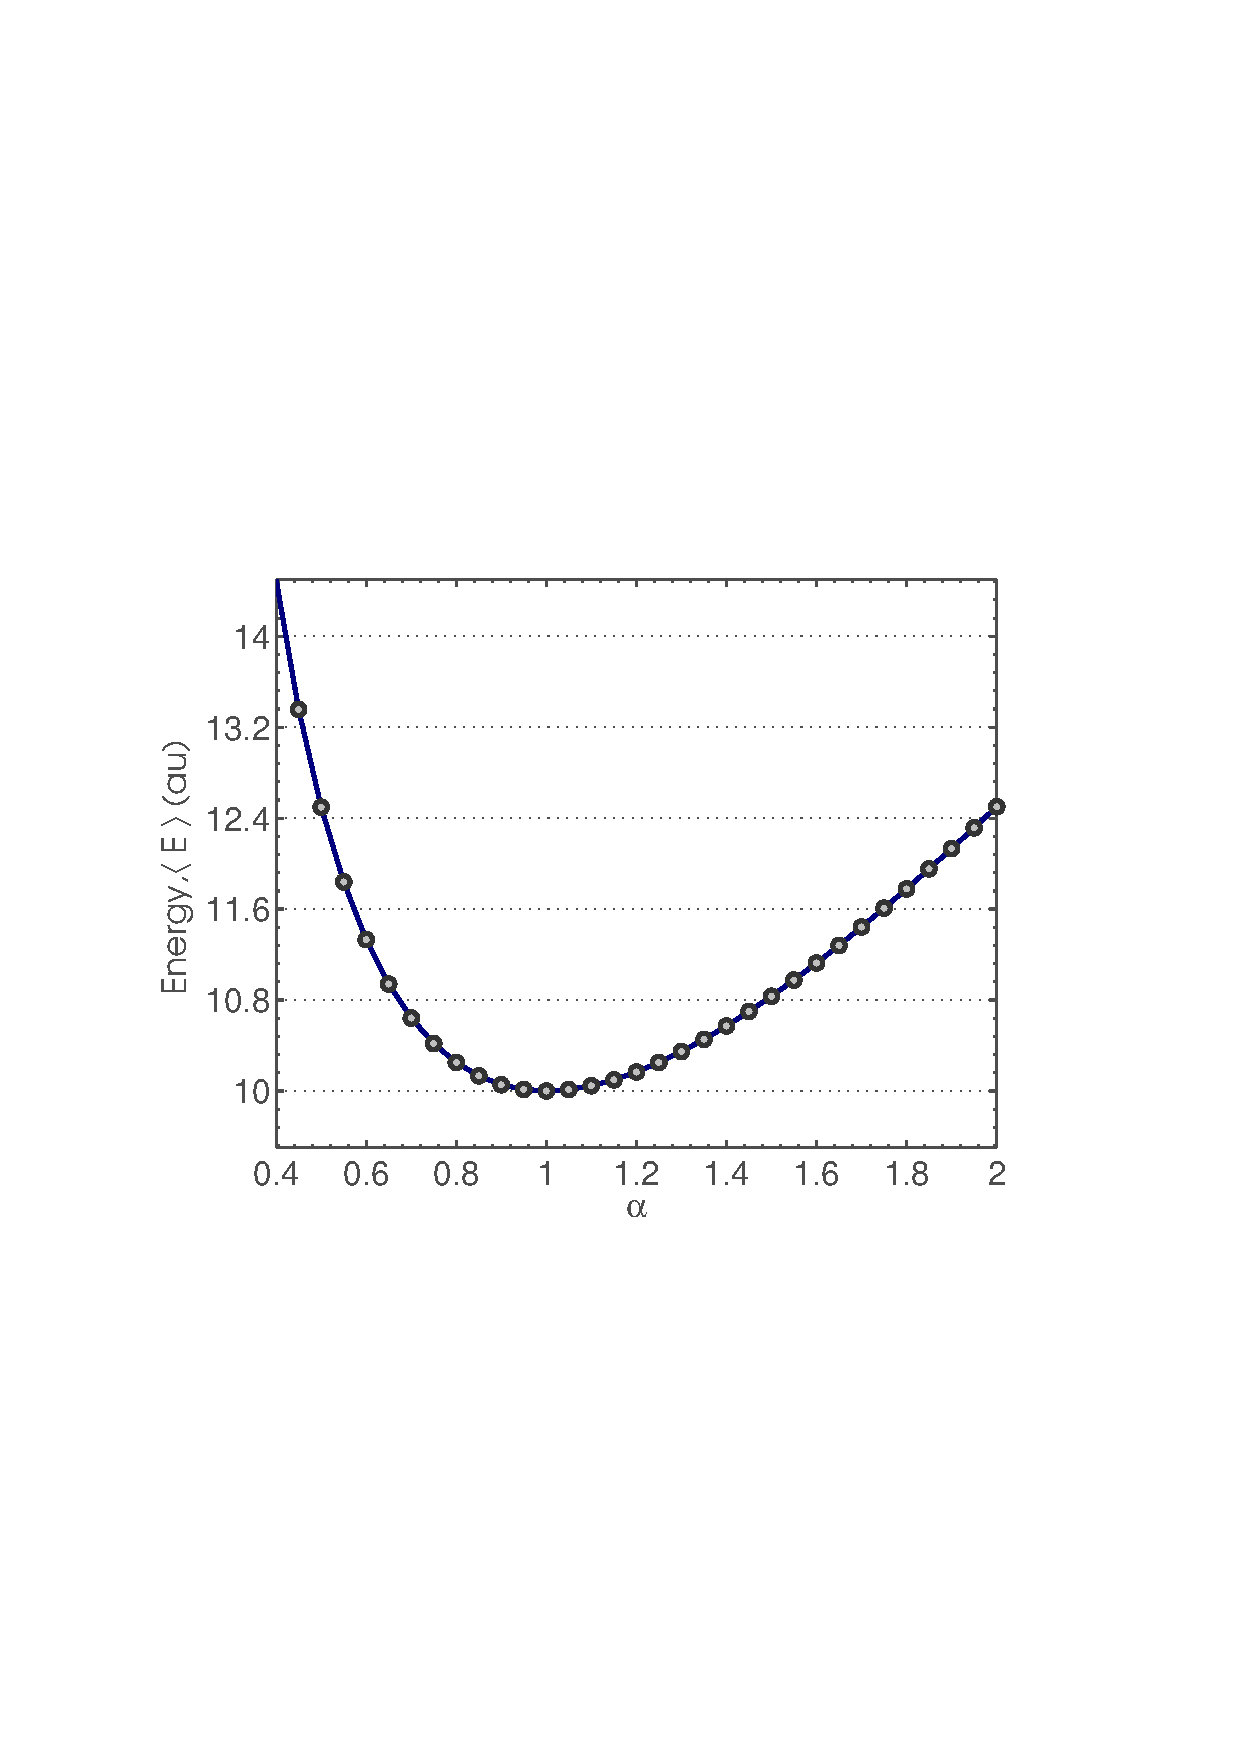
\includegraphics{figures/experimentalData/secondPart/alphaStudy/alpha2DHO6e}}\\      
      \end{tabular}
    \caption{Dependence of the energy on the parameter $\alpha$ for He(left) and Be(right) atoms.}
    \label{alphaHeBe}
  \end{center}
  \end{figure}
\end{frame}


\begin{frame}{Analytical GS for quantum dots (without correlation)}
  \begin{figure}
    \begin{center}
       \begin{tabular}{cc}
      \resizebox{55mm}{!}{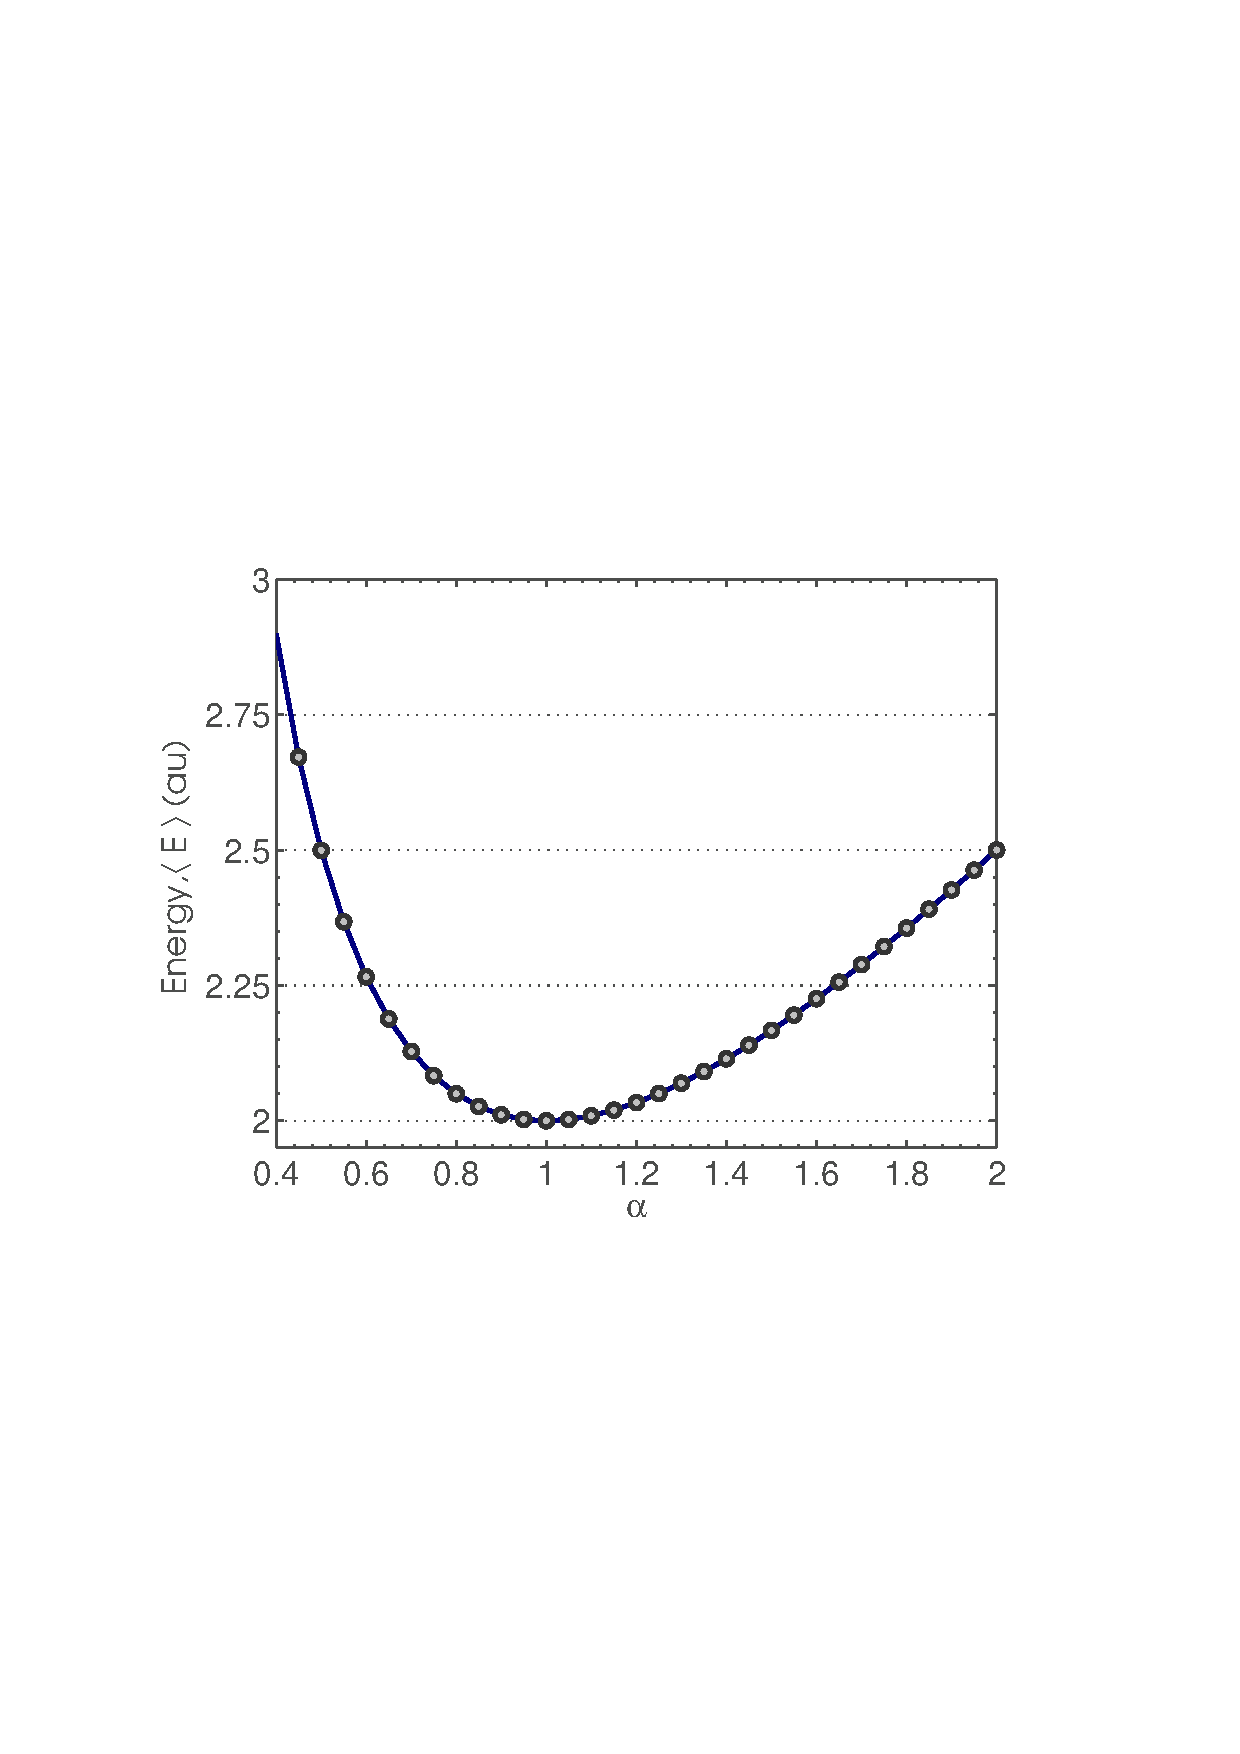
\includegraphics{figures/experimentalData/secondPart/alphaStudy/alpha2DHO2e}} &
      \resizebox{55mm}{!}{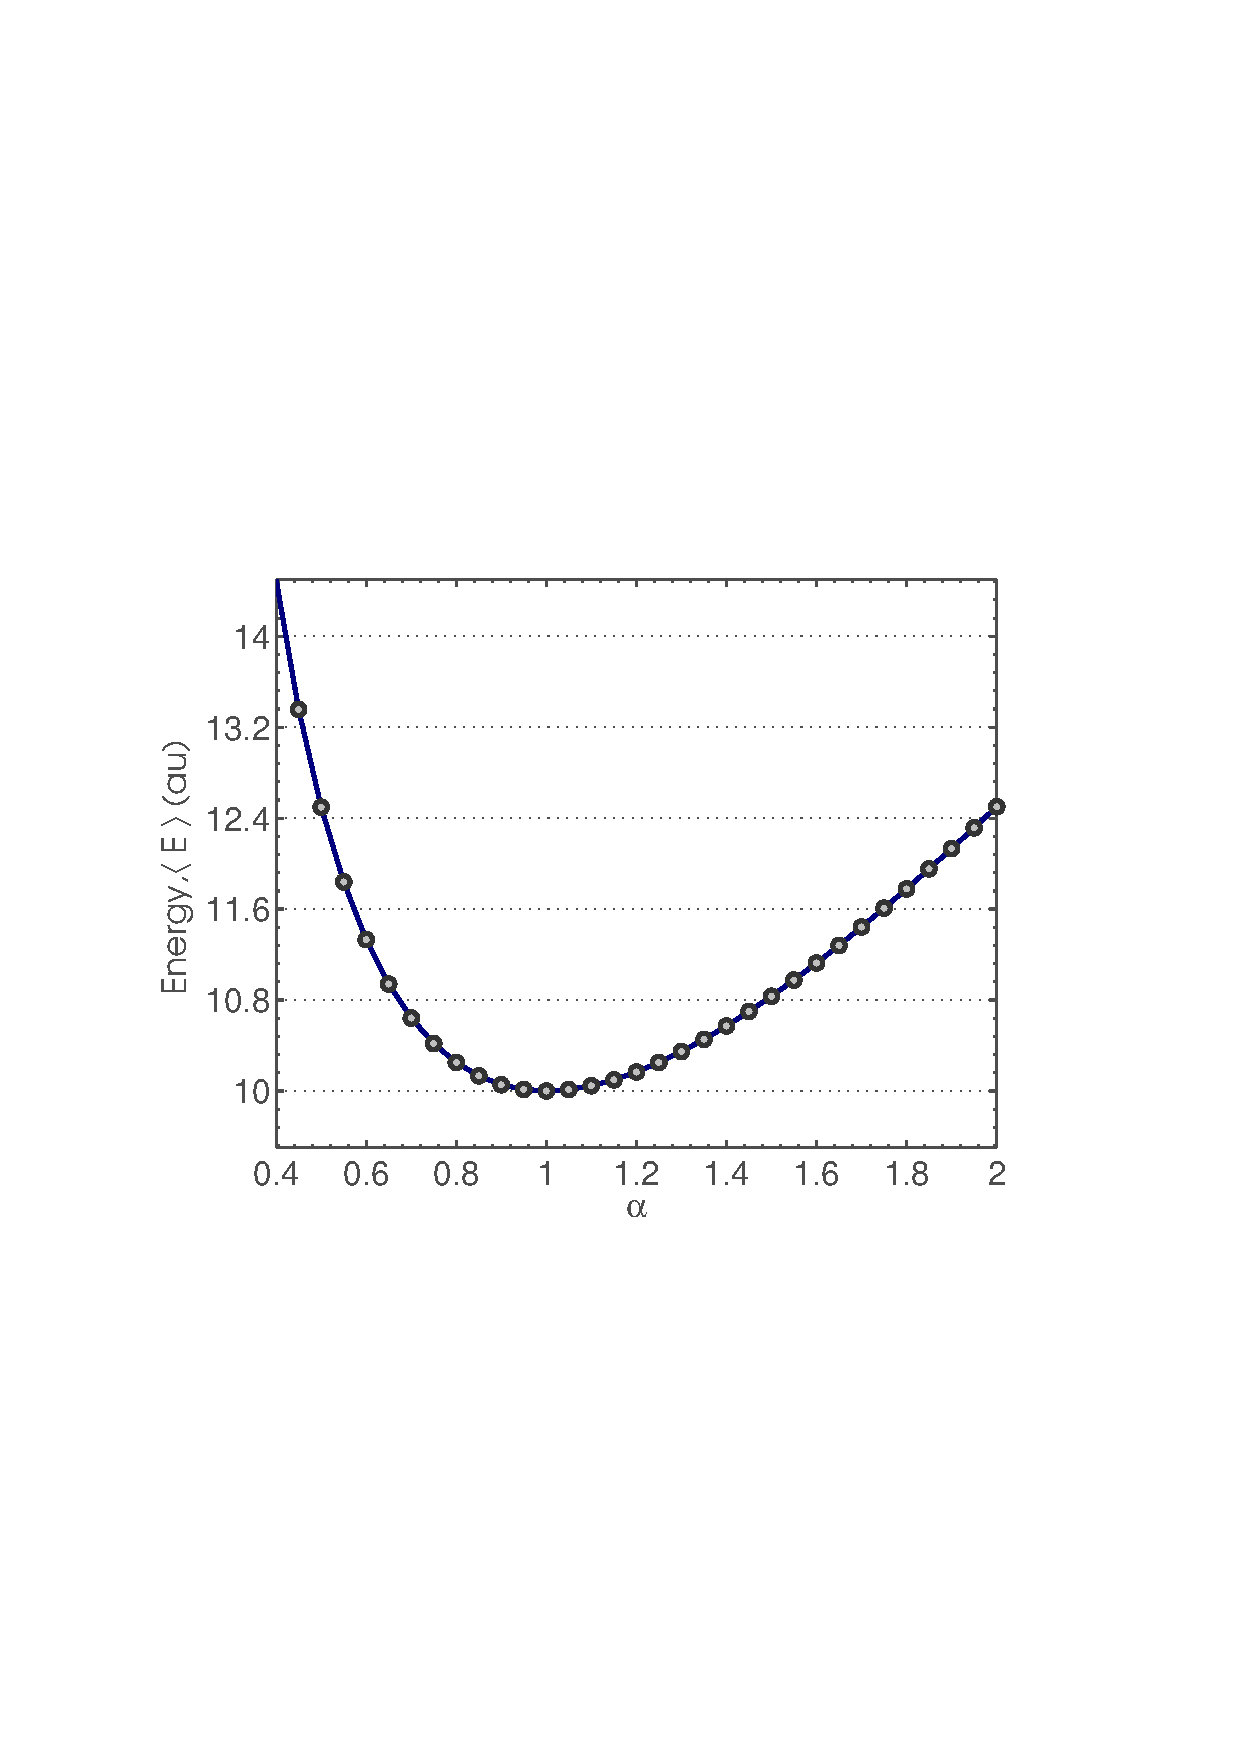
\includegraphics{figures/experimentalData/secondPart/alphaStudy/alpha2DHO6e}}\\
       \end{tabular}
      \caption{Dependence of the energy on the parameter $\alpha$ for a two dimensional harmonic oscillator with two and six electrons electrons, respectively.}
      \label{alpha2DHO2e6e}
    \end{center}
  \end{figure}

\end{frame}



\begin{frame}{Graphical estimation of the GS energy for atoms}
  \begin{figure}[!hbt]
    \begin{center}
      \begin{tabular}{cc}
        \resizebox{55mm}{!}{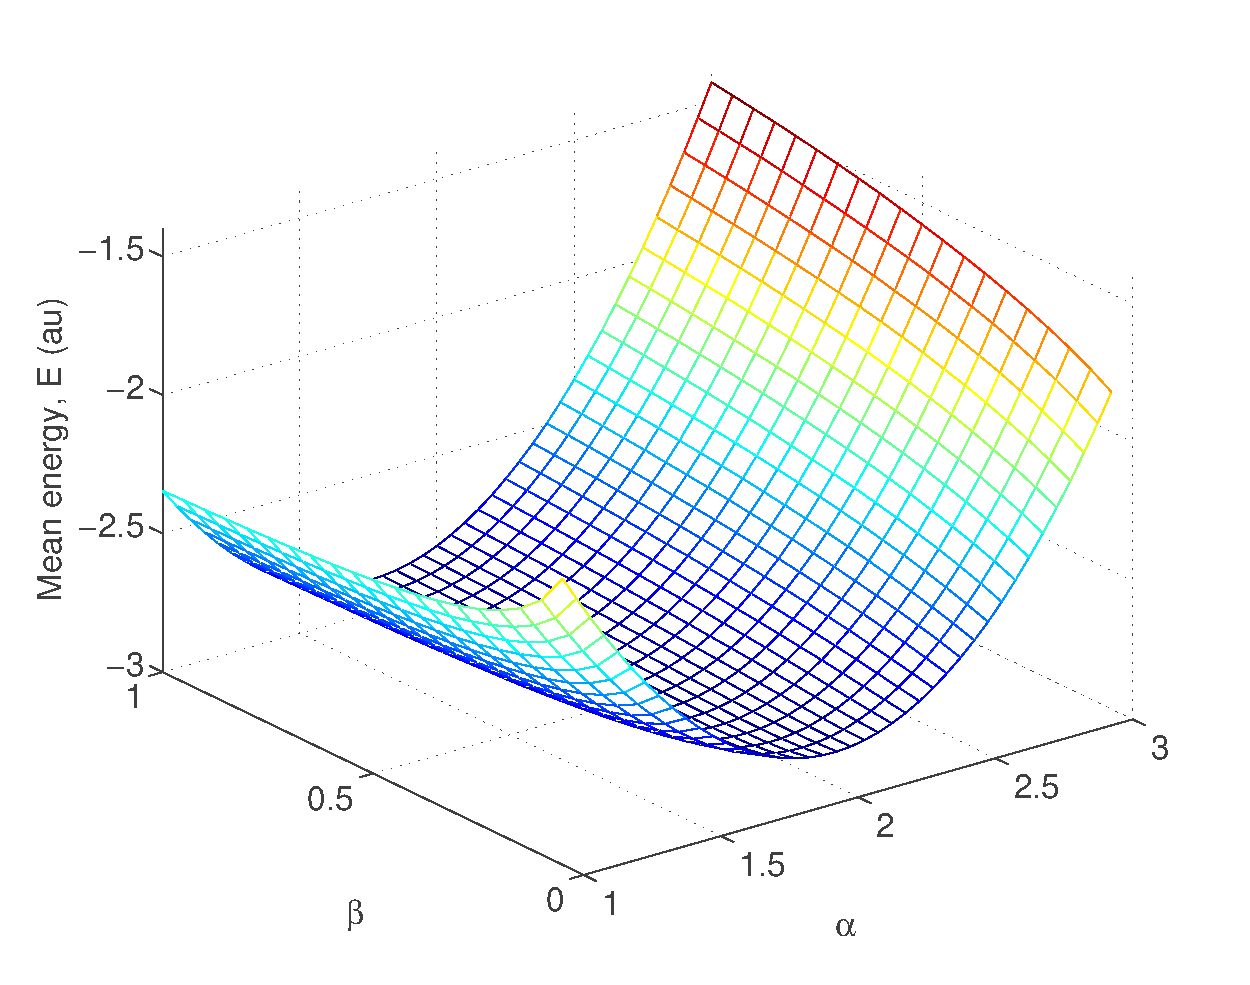
\includegraphics{figures/experimentalData/secondPart/alphaBetaStudy/plot3DAlphaBetaHe}} &
        \resizebox{55mm}{!}{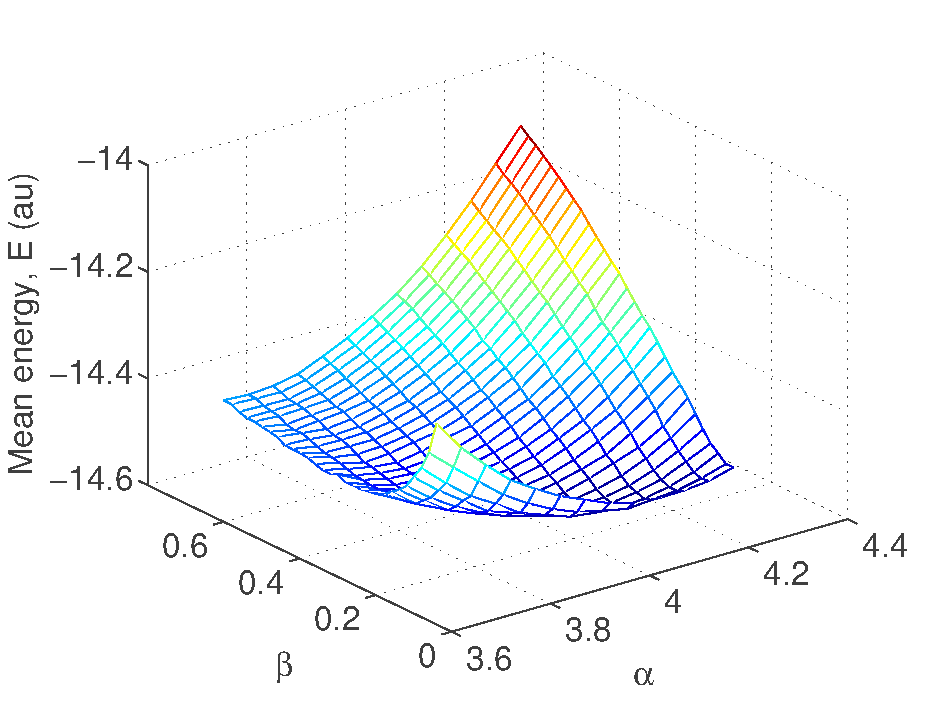
\includegraphics{figures/experimentalData/secondPart/alphaBetaStudy/plot3DAlphaBetaBeSim1}}\\
      \label{alphaBetaHe}
      \end{tabular}
      \caption{Dependence of the energy on the parameters $\alpha$ and $\beta$ for He and Be atoms. Experiment was carried out with $10^7$ Monte Carlo cycles, $10 \%$ equilibration steps and $dt = 0.01$.}
    \end{center}
  \end{figure}
  
\end{frame}



\begin{frame}{Graphical estimation of the GS energy for QD}

  \begin{figure}[!hbt]
    \begin{center}
      \begin{tabular}{cc}
        \resizebox{58mm}{!}{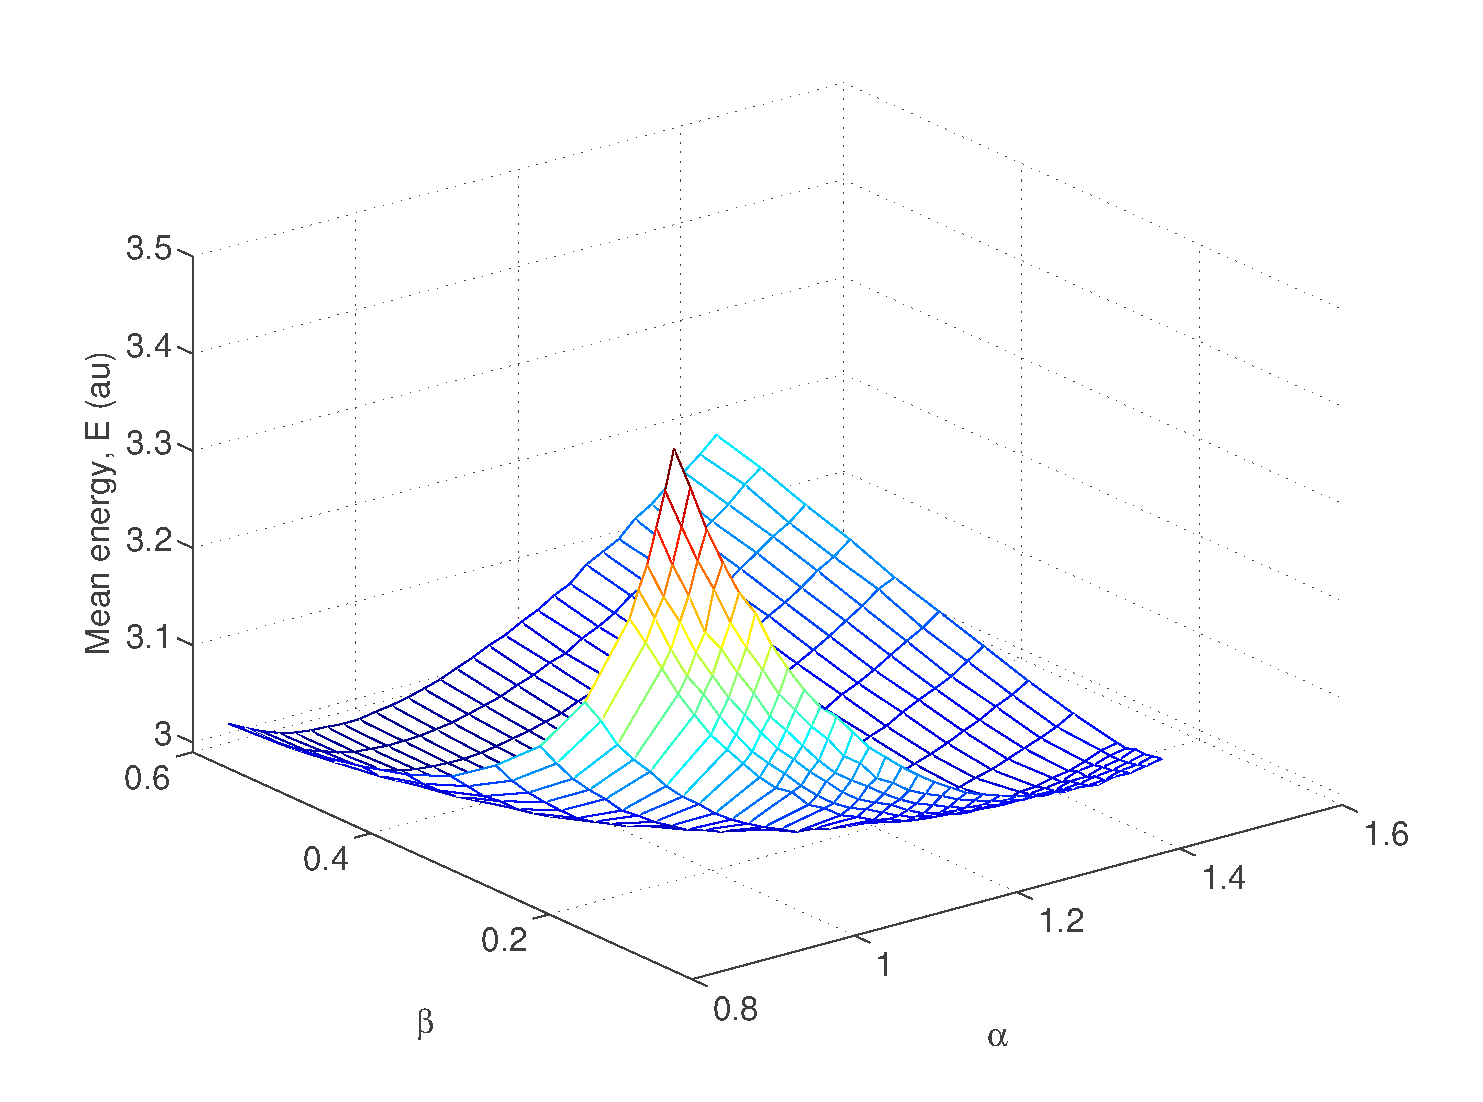
\includegraphics{figures/experimentalData/secondPart/alphaBetaStudy/plotAlphaBeta2DQDot2e}} &
        \resizebox{50mm}{!}{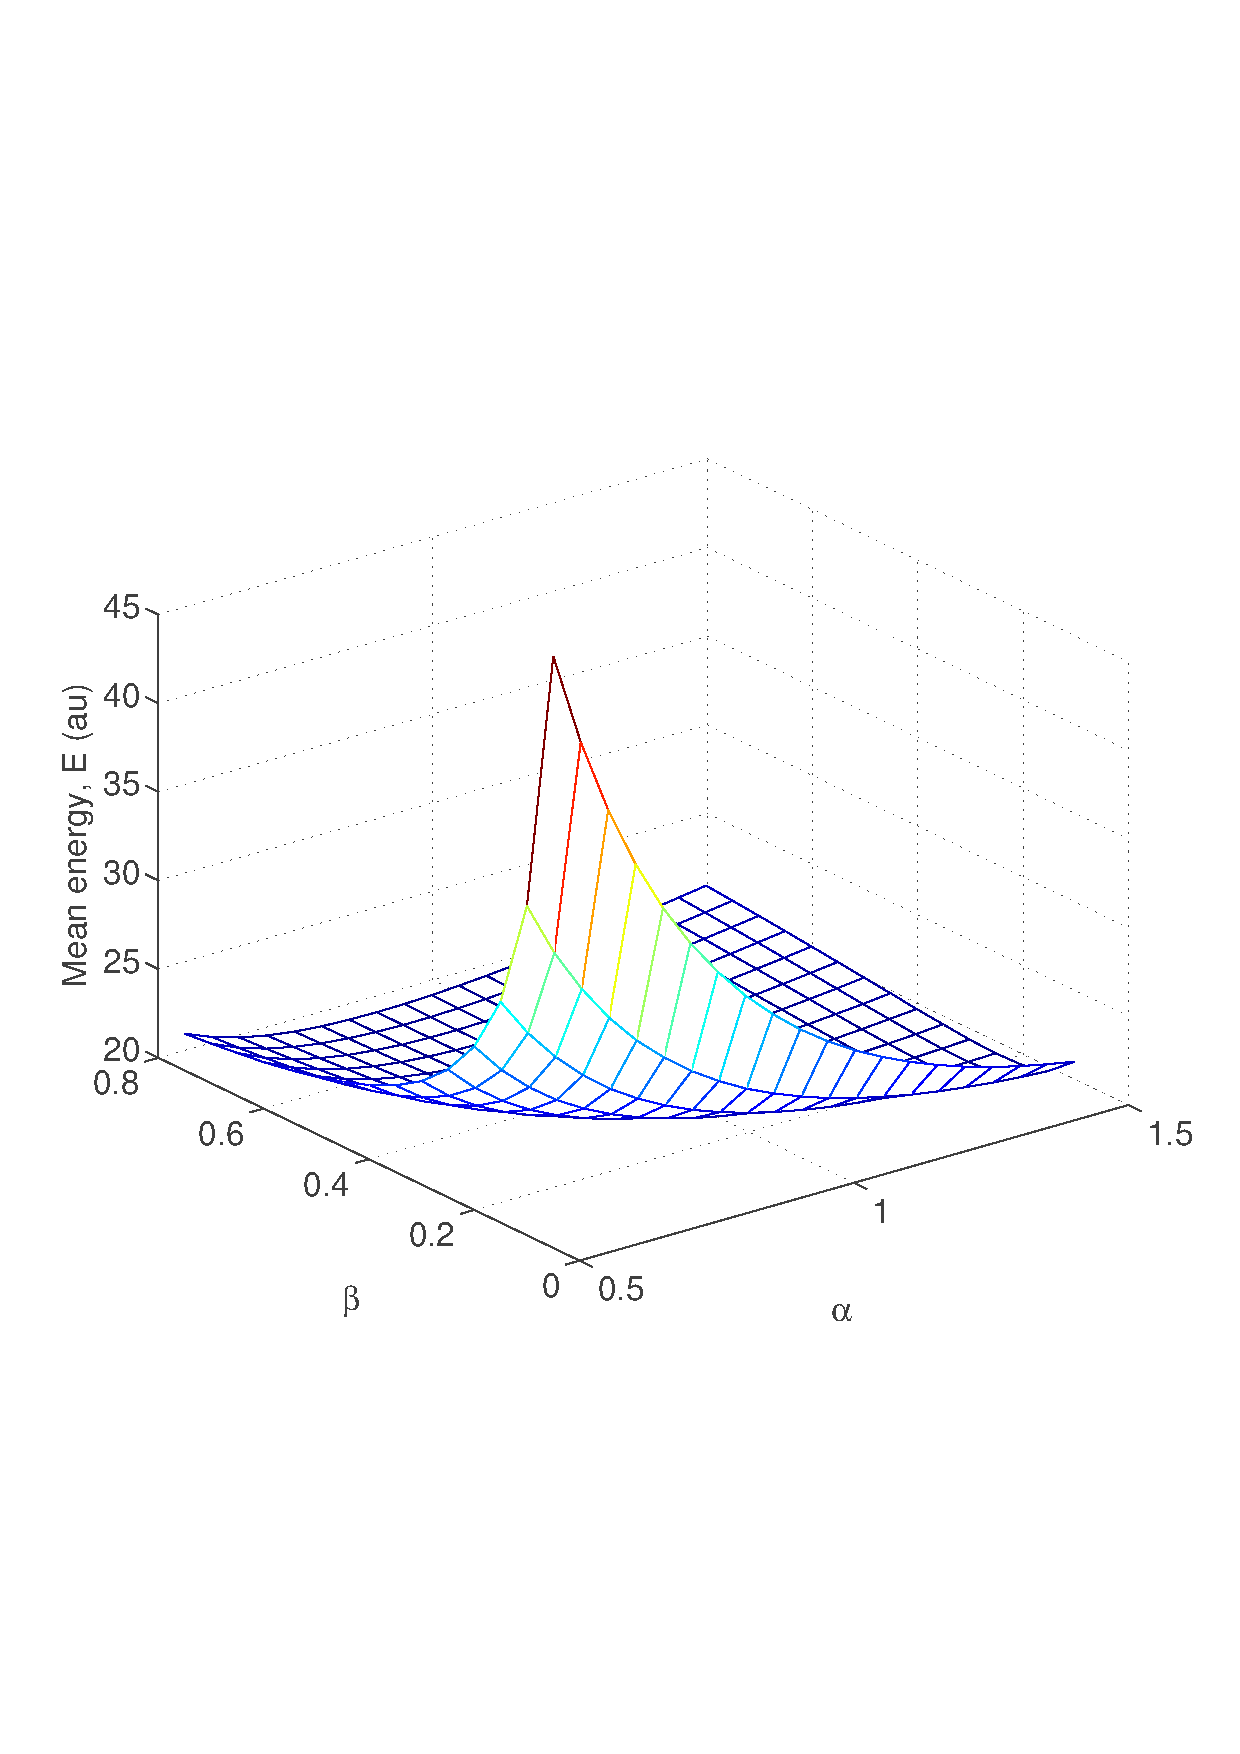
\includegraphics{figures/experimentalData/secondPart/alphaBetaStudy/alphaBeta}} \\
        \label{alphaBetaHe}
        \end{tabular}
       \caption{Dependence of the energy on the parameters $\alpha$ and $\beta$ for a two-dimensional quantum dots with two and electrons, respectively. Experiment was carried out with $10^7$ Monte Carlo cycles, $10 \%$ equilibration steps and $dt = 0.01$.}
    \end{center}
  \end{figure}
 
\end{frame}

  
\begin{frame}{Graphical estimation of the GS energy for helium}  
  \begin{scriptsize}
  \begin{figure}[!hbt]
    \begin{center}
       \begin{tabular}{cc}
      \resizebox{55mm}{!}{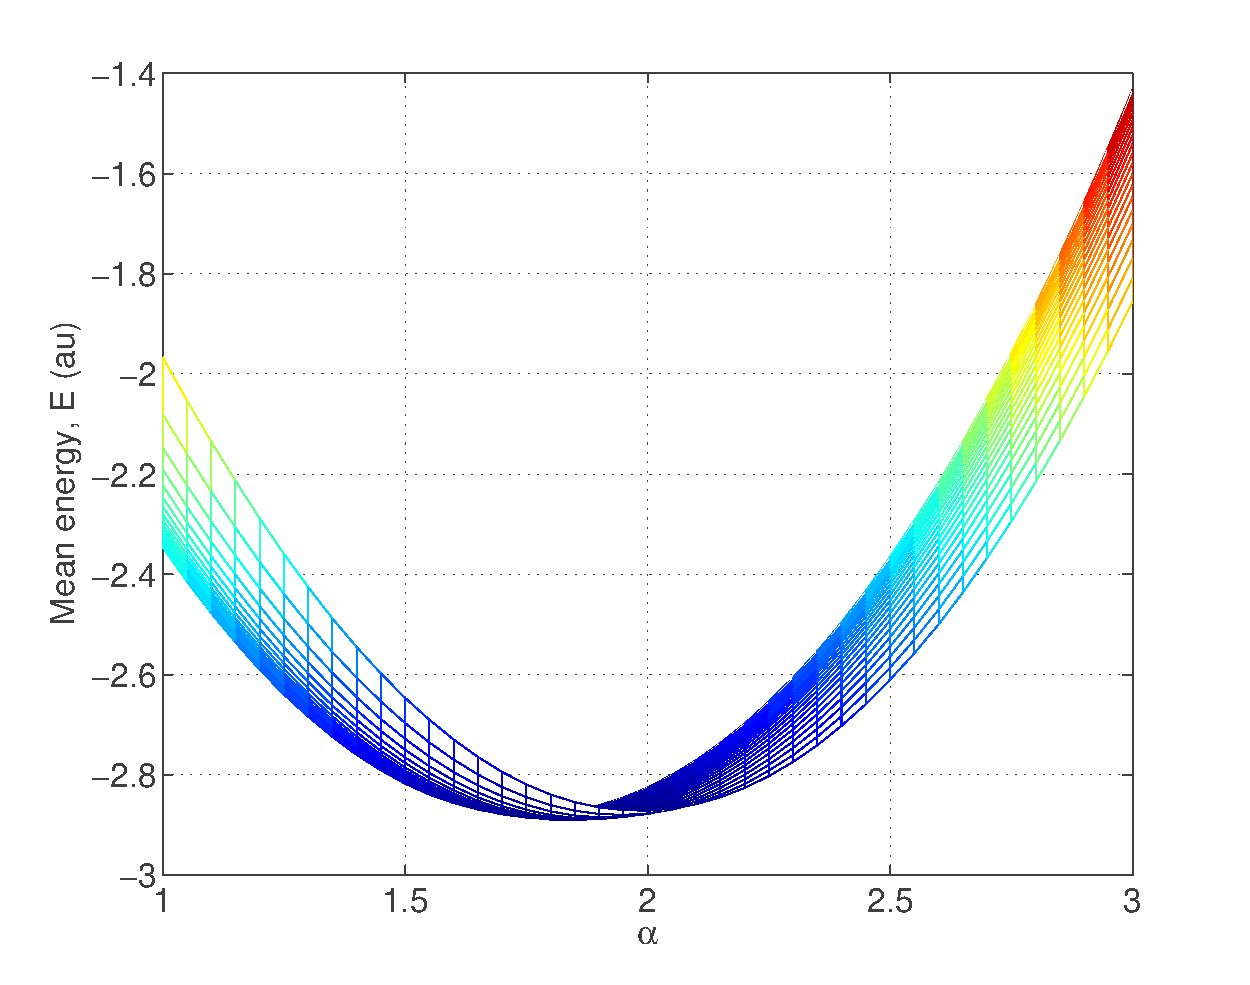
\includegraphics{figures/experimentalData/secondPart/alphaBetaStudy/zoomAlphaHe}}&%%%alphaBetaStudies/alphaZoomHe}} &
      \resizebox{55mm}{!}{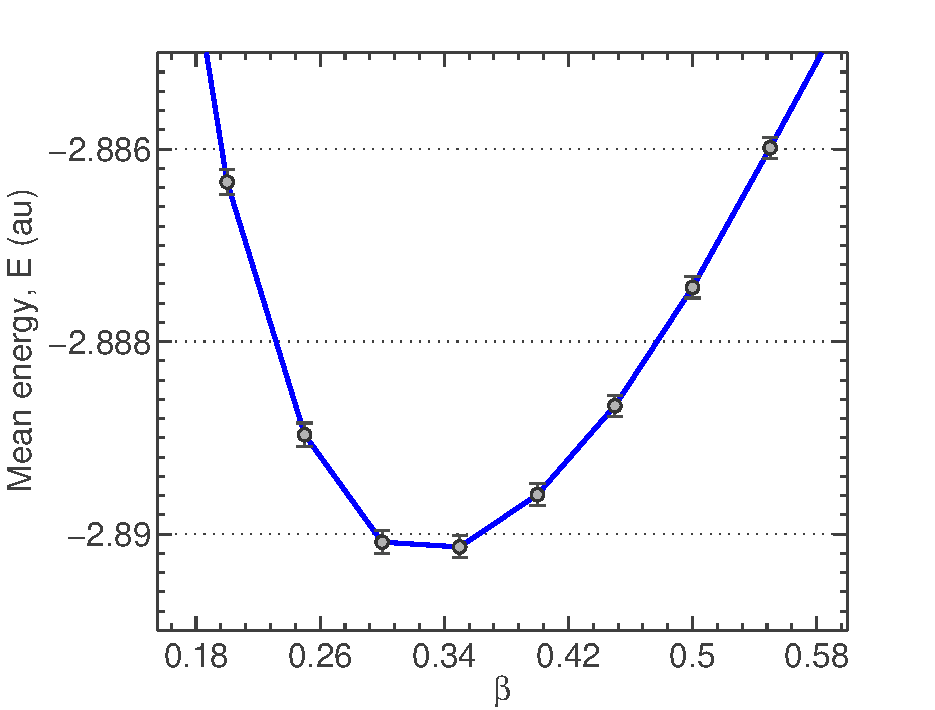
\includegraphics{figures/experimentalData/secondPart/alphaBetaStudy/minBetaFixedAlphaHe}}\\%%%%alphaBetaStudies/minBetaHeFixedAlpha1_85}}\\
       \end{tabular}
      \caption{Dependence of the energy on $\alpha$ (left) along the value of $\beta$ (right) that gives the minimum variational energy for a He atom.}
      \label{alphaHe}
    \end{center}
  \end{figure}
  \end{scriptsize}

\end{frame}





\begin{frame}{Graphical estimation of the GS energy for beryllium}
  \begin{figure}[!hbt]
  \begin{center}
    \begin{tabular}{cc}
      \resizebox{55mm}{!}{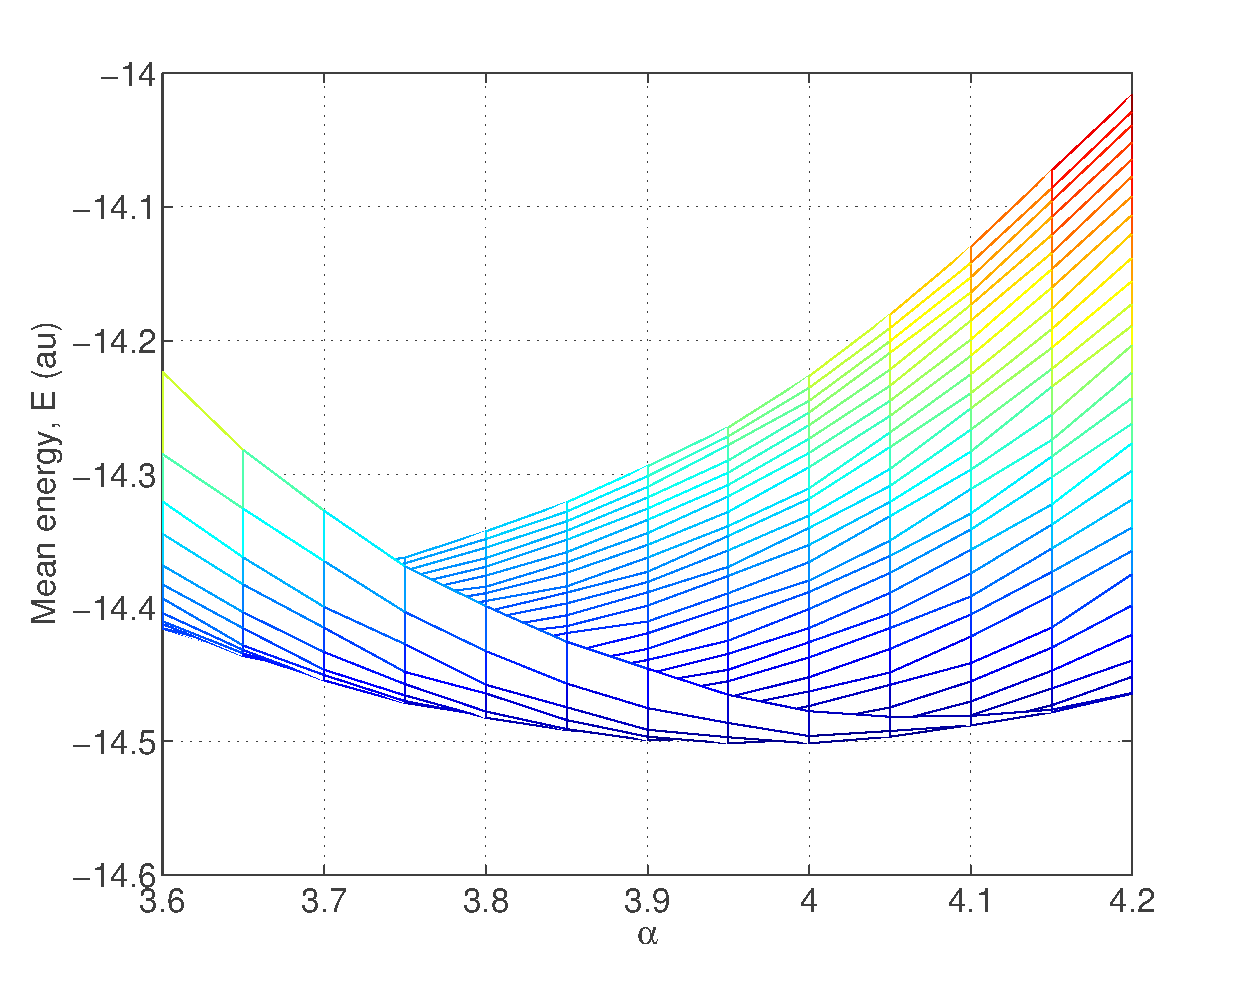
\includegraphics{figures/experimentalData/secondPart/alphaBetaStudy/zoomAlphaBeSim1}}&
      \resizebox{55mm}{!}{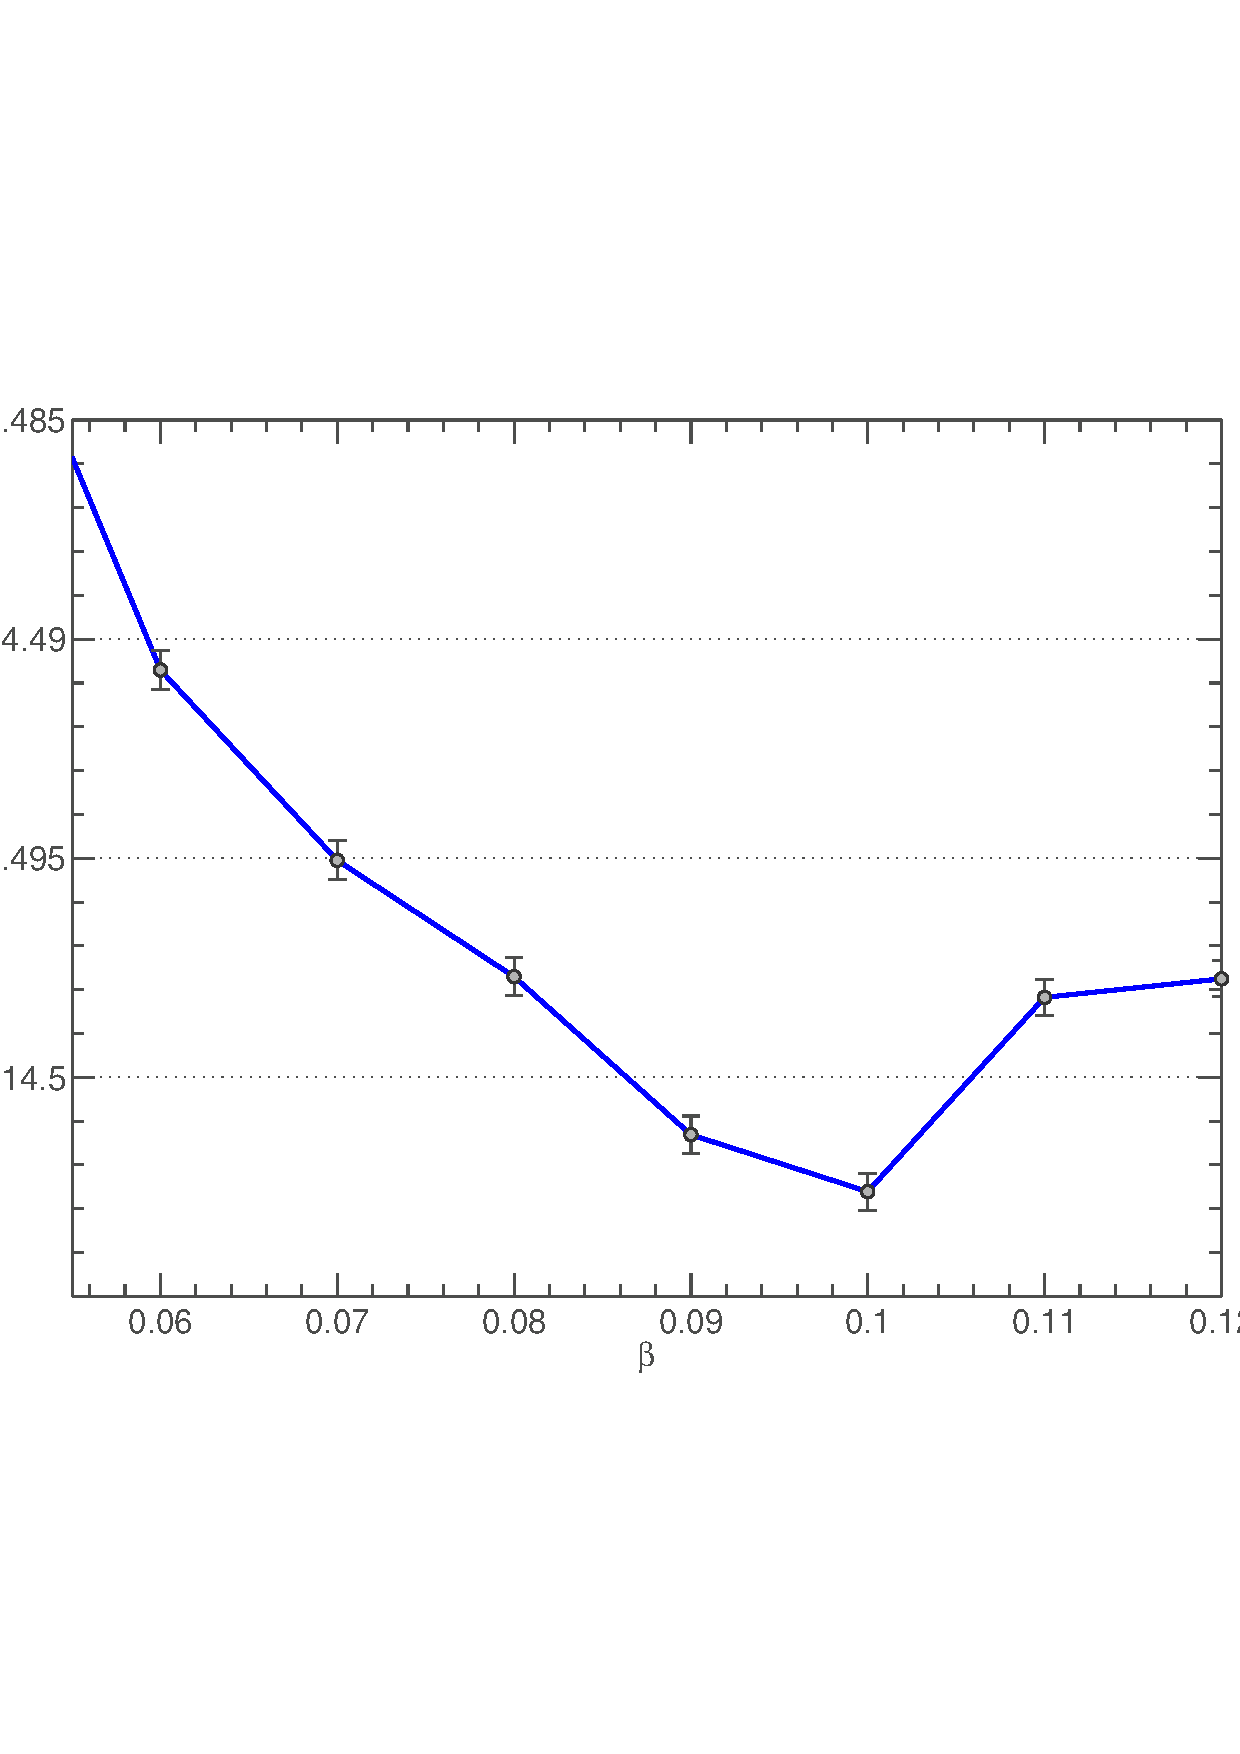
\includegraphics{figures/experimentalData/secondPart/alphaBetaStudy/minBetaFixedAlphaBeSim2}}\\
    \end{tabular}
    \caption{Dependence of the energy on $\alpha$ (left) along the value of $\beta$ (right) that gives the minimum variational energy for a Be atom.}
  \end{center}
  \end{figure}
\end{frame}




\begin{frame}{Graphical estimation of the GS energy for 2-$e^-$ QD}
  \begin{figure}[!hbt]
    \begin{center}
       \begin{tabular}{cc}
        \resizebox{55mm}{!}{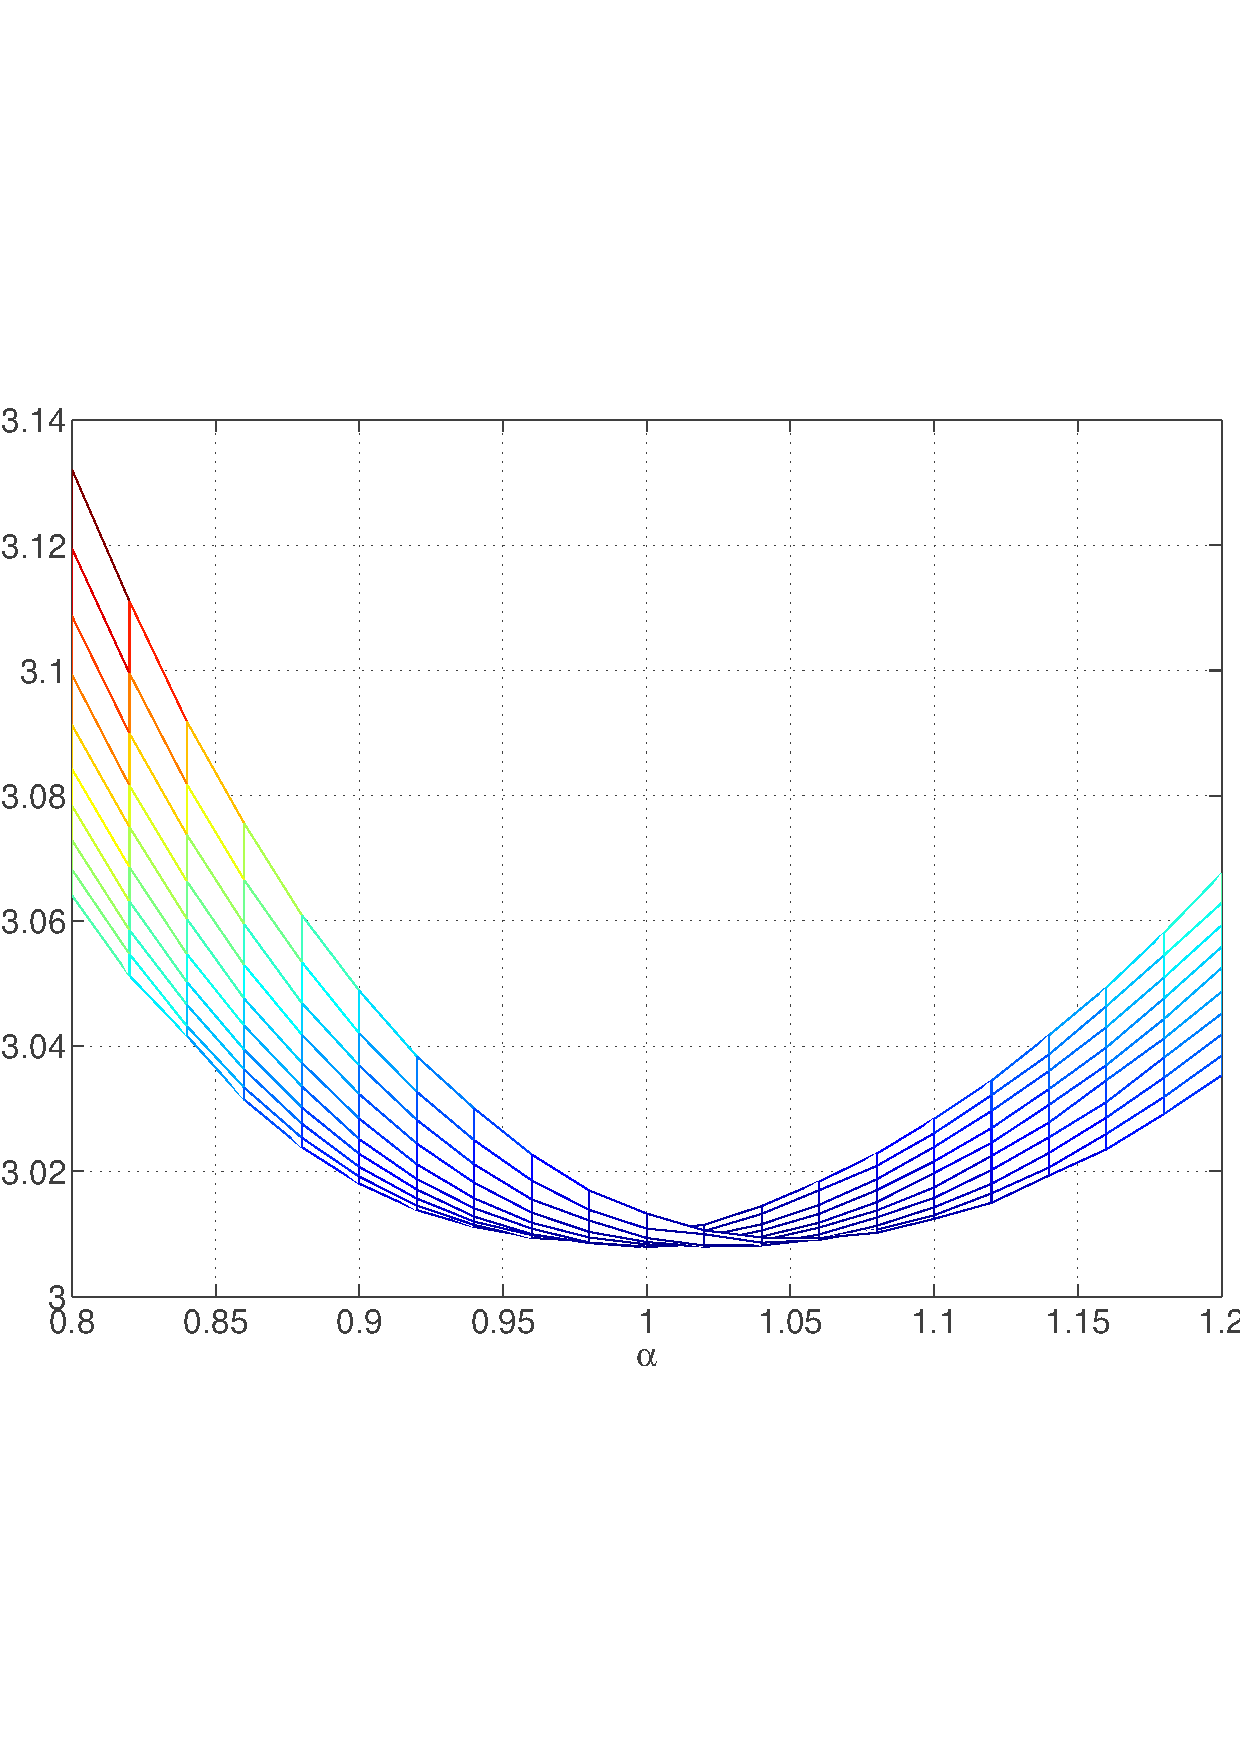
\includegraphics{figures/experimentalData/secondPart/alphaBetaStudy/zoomAlpha2DQDot2e}} &
        \resizebox{55mm}{!}{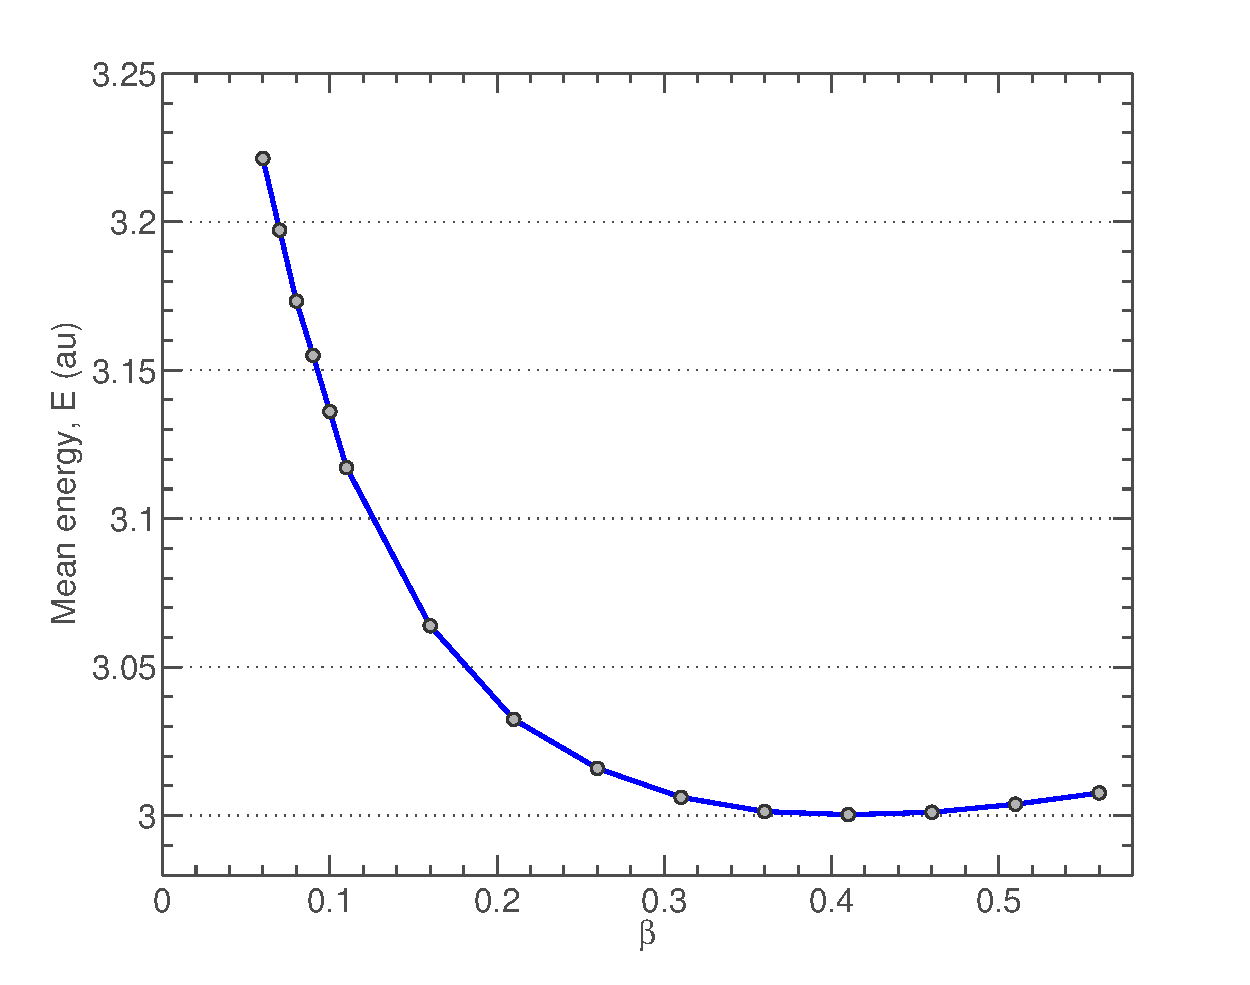
\includegraphics{figures/experimentalData/secondPart/alphaBetaStudy/zoomBeta2DQDot2e}}\\
      \end{tabular}
      \caption{Dependence of the energy on $\alpha$ (left) along the value of $\beta$ (right) that gives the minimum variational energy for a two-dimensional quantum dot with two electrons.}
      \label{alpha2DHO2e}
    \end{center}
  \end{figure}
\end{frame}


\begin{frame}{Graphical estimation of the GS energy for 6-$e^-$ QD}
  \begin{figure}[!hbt]
    \begin{center}
       \begin{tabular}{cc}
      \resizebox{55mm}{!}{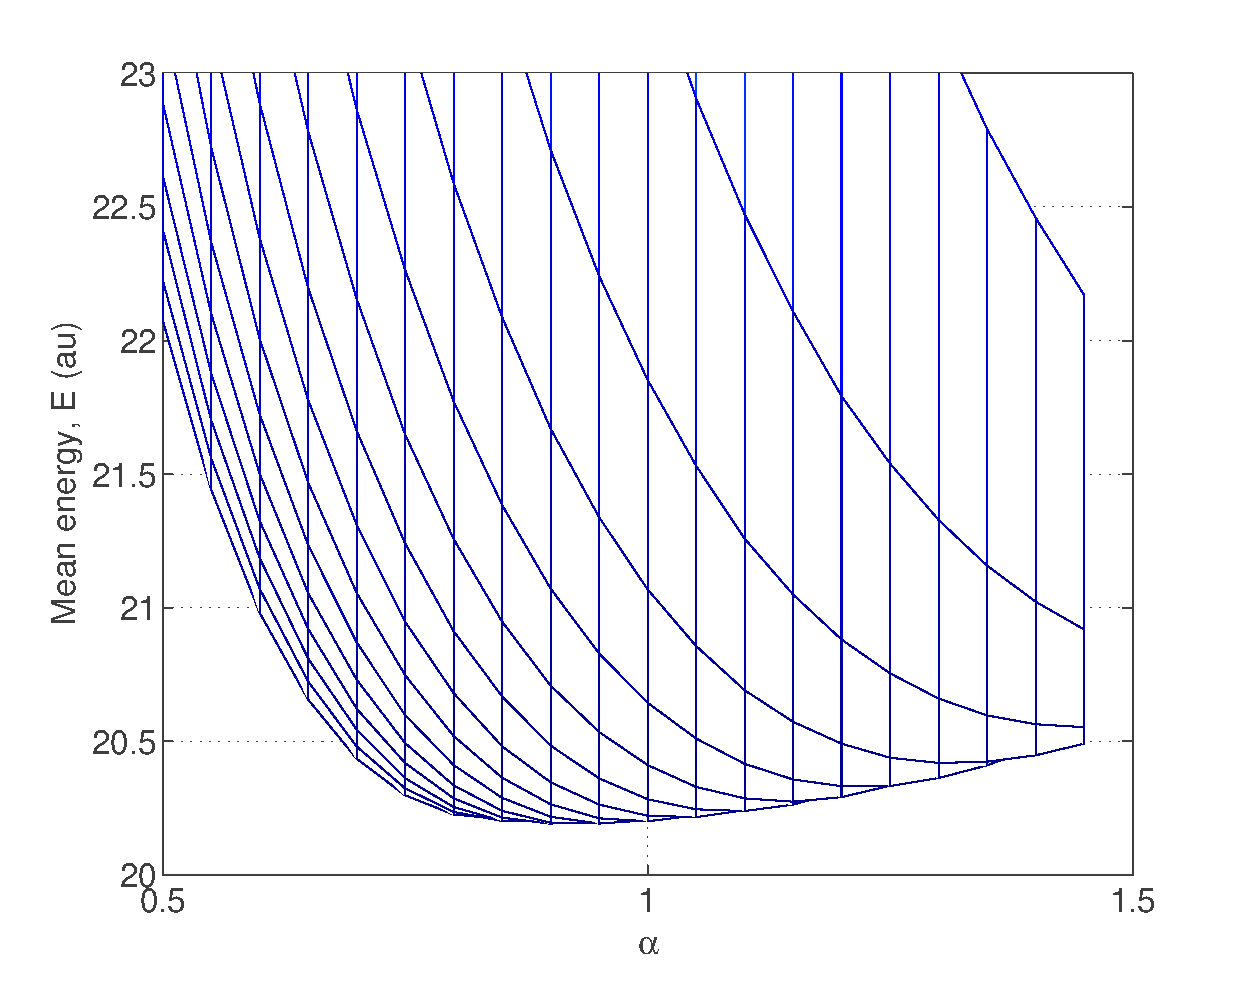
\includegraphics{figures/experimentalData/secondPart/alphaBetaStudy/zoomAlpha}} &
      \resizebox{55mm}{!}{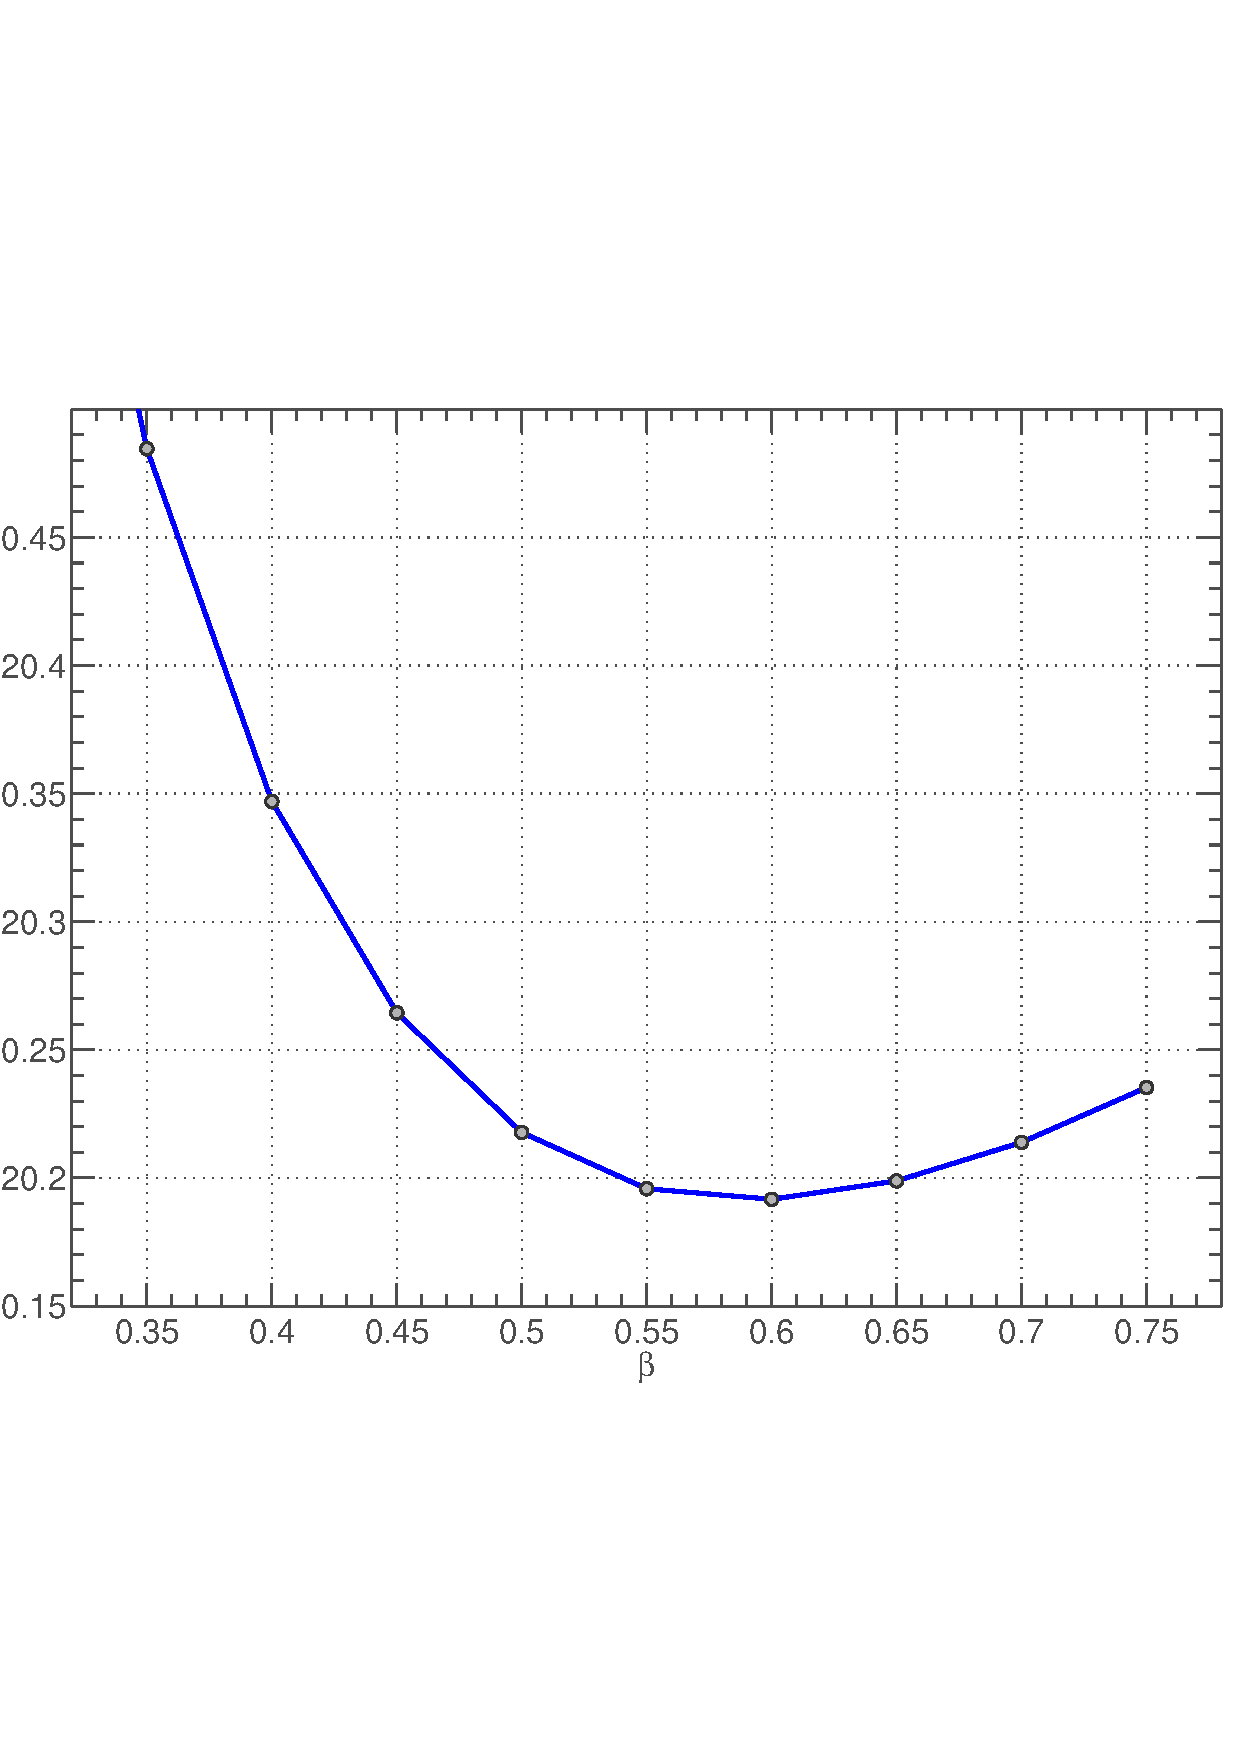
\includegraphics{figures/experimentalData/secondPart/alphaBetaStudy/zoomBeta}}\\
       \end{tabular}
      \caption{Dependence of the energy on $\alpha$ (left) along the value of $\beta$ (right) that gives the minimum variational energy for a two-dimensional quantum dot with six electrons.}
      \label{alpha2DHO6e}
    \end{center}
  \end{figure}

\end{frame}

\begin{frame}{Summary of the results with graphical estimation}
  \begin{scriptsize}
  \begin{table}[!hbt]
  \centering
    \begin{tabular}{lcccr}
      \toprule[1pt]
      \textbf{System} & $\alpha_{optimal}$ & $\beta_{optimal}$ & \textbf{Energy}, $\langle E \rangle$ (au) \\
      \midrule[1pt]
      He      &  1.85   &   0.35  & $-2.8901 \pm 1.0 \times 10{-4}$ \\
      Be      &  3.96   &   0.09  & $-14.5043 \pm 4.0 \times 10^{-4}$\\
      2DQDot2e ($\omega=1.0$) & 0.98  & 0.41  & $3.0003 \pm 1.2 \times 10^{-5}$ \\
      %%%2DQDot6e ($\omega = 1.0$)  & 1.03   & 0.18 & $20.2180 \pm 4.0 \times 10^{-4}$\\
      2DQDot6e ($\omega = 1.0$) & 0.9   & 0.6 & $20.19 \pm 1.2 \times 10^{-4}$\\
      \bottomrule[1pt]
    \end{tabular}\caption{Ground state energy and corresponding variational parameters  $\alpha$ and $\beta$ estimated graphically. (2DQDot2e stands for two-dimensional quantum dot with two electrons).}
    \label{energiesWithGraphPar}
  \end{table}
  \end{scriptsize}
\end{frame}

\subsection{Optimization of the trial wave function}
\begin{frame}{Optimization with Quasi-Newton method}

  \begin{scriptsize}
  \begin{table}[!hbt]
  \centering
  \begin{tabular}{lccccrcc}
    \toprule[1pt]
    \textbf{System} & $\alpha_{0}$ & $\beta_{0}$ & $\alpha_{opt}$ & $\beta_{opt}$ &\textbf{Energy}, (au)\\
    \midrule[1pt]
    He              & 1.564  & 0.134    & 1.838   &  0.370  & -2.891   \\
    Be              & 3.85  & 0.08    & 3.983   &  0.104  &   -14.503  \\
    \bottomrule[1pt]
  \end{tabular}\caption{Optimized variational parameters and corresponding energy minimization using a quasi-Newton method. Simulation parameters: $10^7$ Monte Carlo cycles with 10 \% equilibration steps, $dt = 0.01$.}\label{optizedQuasiNewtonParameters}
  \end{table}
  \end{scriptsize}

\end{frame}




\begin{frame}{Convergence to the optimal parameters for helium}
  \begin{scriptsize}
  \begin{figure}[!hbt]
    \begin{center}
      \begin{tabular}{cc}
        \resizebox{50mm}{!}{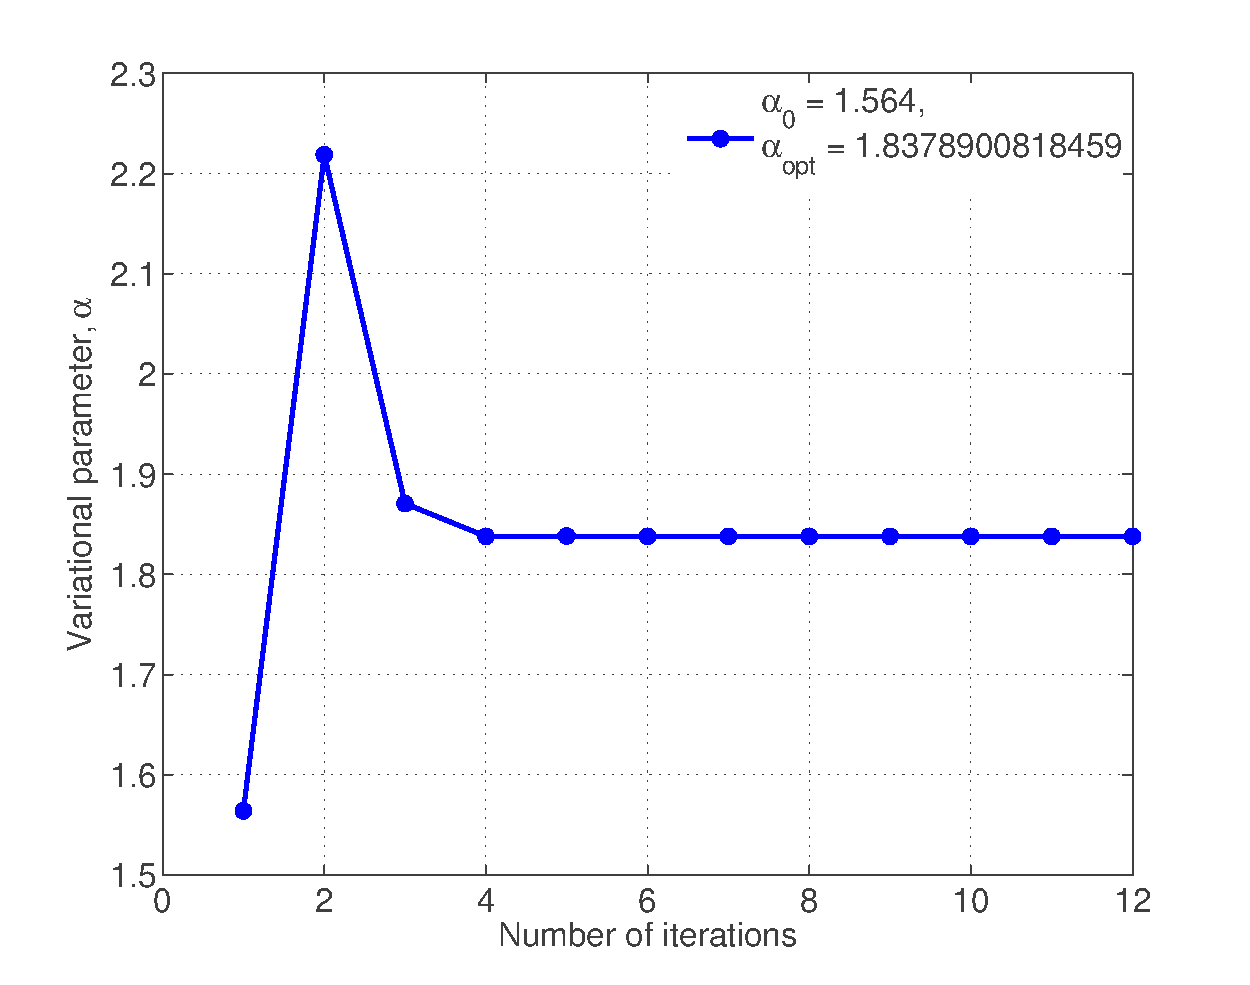
\includegraphics{figures/experimentalData/quasiNewtonOptimization/plotAlphaEvolHe}}&
        \resizebox{50mm}{!}{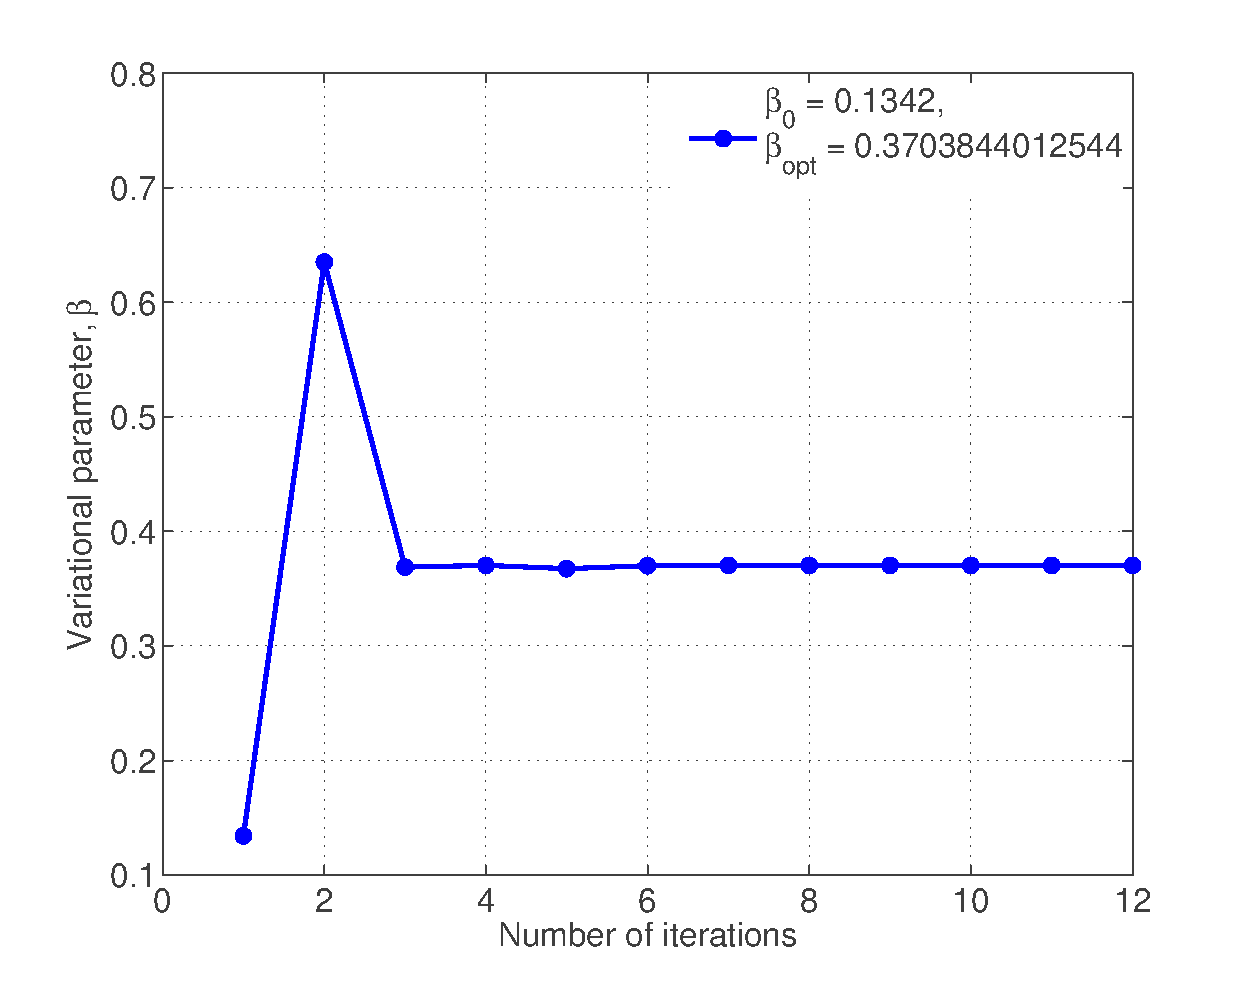
\includegraphics{figures/experimentalData/quasiNewtonOptimization/plotBetaEvolHe}}\\
      \end{tabular}
      \caption{Evolution of the variational parameters $\alpha$ and $\beta$ as a function of the number of iterations during the optimization of the trial wave function of He atom with quasi-Newton method. The experiment was carried out with $10^7$ Monte Carlo cycles and $10 \%$ equilibration steps in four nodes.}
    \end{center}
  \end{figure}
  \end{scriptsize}  
\end{frame}




\begin{frame}{Convergence to the minimal energy for helium}
  \begin{scriptsize}
  \begin{figure}[!hbt]
    \begin{center}
      \resizebox{60mm}{!}{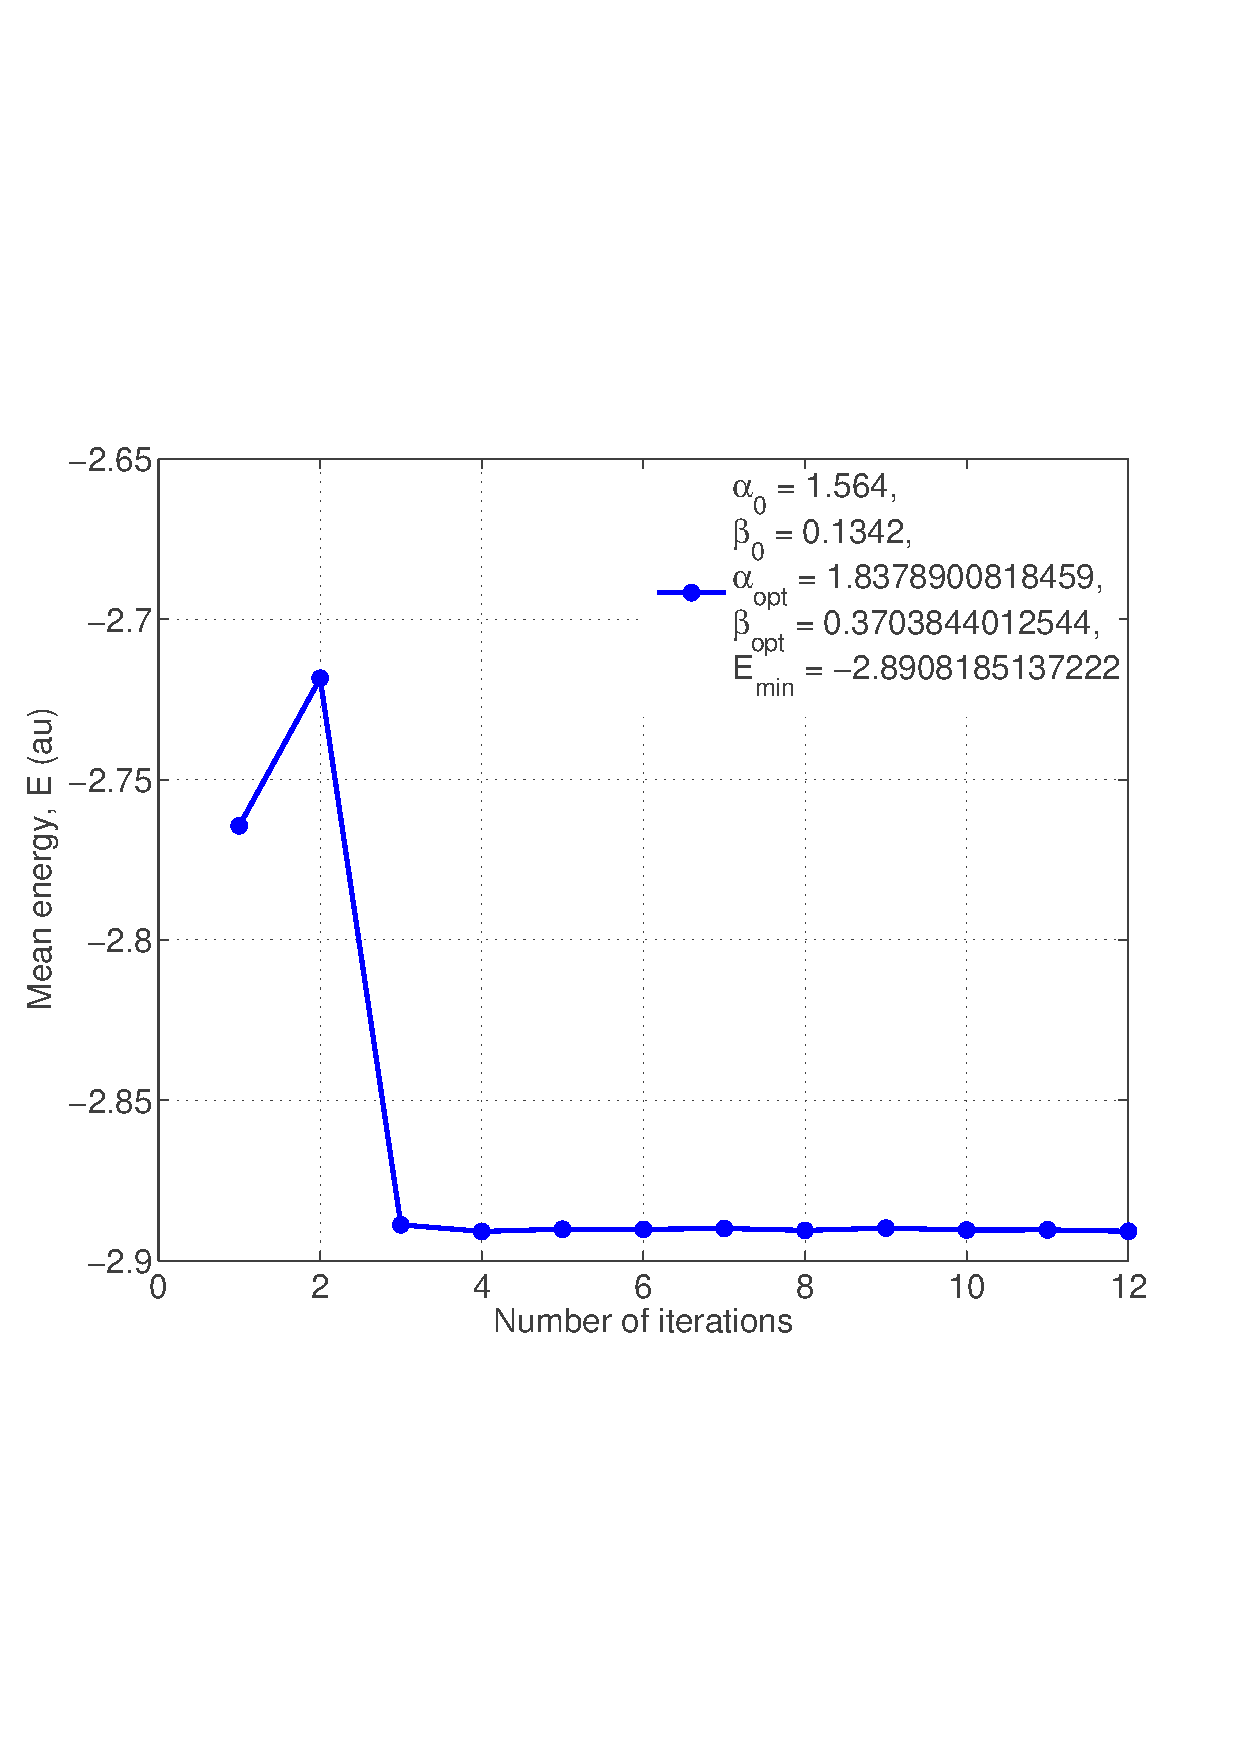
\includegraphics{figures/experimentalData/quasiNewtonOptimization/plotOptAlphaBetaEnergyHe}}\\
      \caption{Evolution of the energy as a function of the number of iterations during the optimization of the trial wave function of He atom with the quasi-Newton method. The experiment was carried out with $10^7$ Monte Carlo cycles and $10 \%$ equilibration steps in four nodes.}
      \label{quasiNewtonOptHe}
    \end{center}
  \end{figure}
  \end{scriptsize}
\end{frame}




\begin{frame}{Convergence to the optimized parameters for Be}
  \begin{scriptsize}
  \begin{figure}[!hbt]
  \begin{center}
    \begin{tabular}{cc}
      \resizebox{55mm}{!}{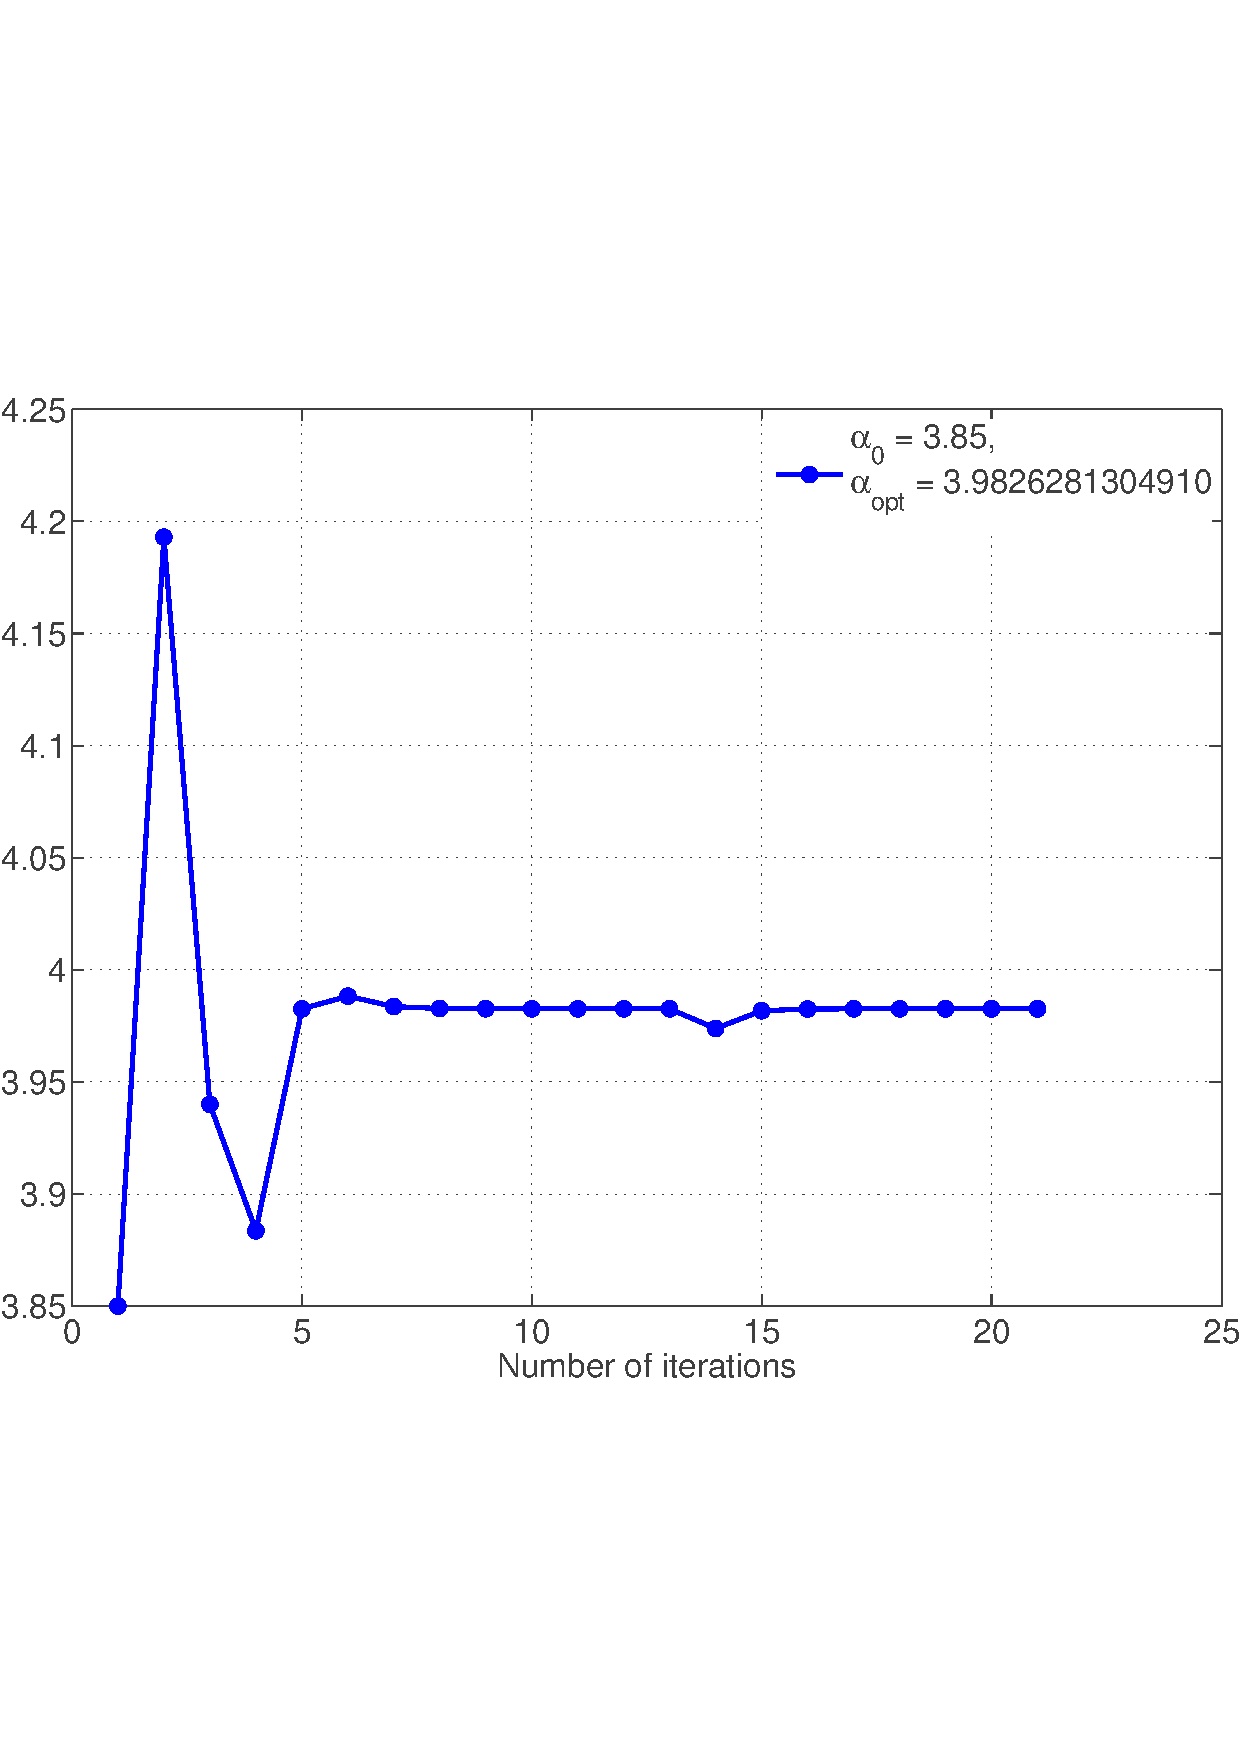
\includegraphics{figures/experimentalData/quasiNewtonOptimization/evolAlphaBeOpt}}&
      \resizebox{55mm}{!}{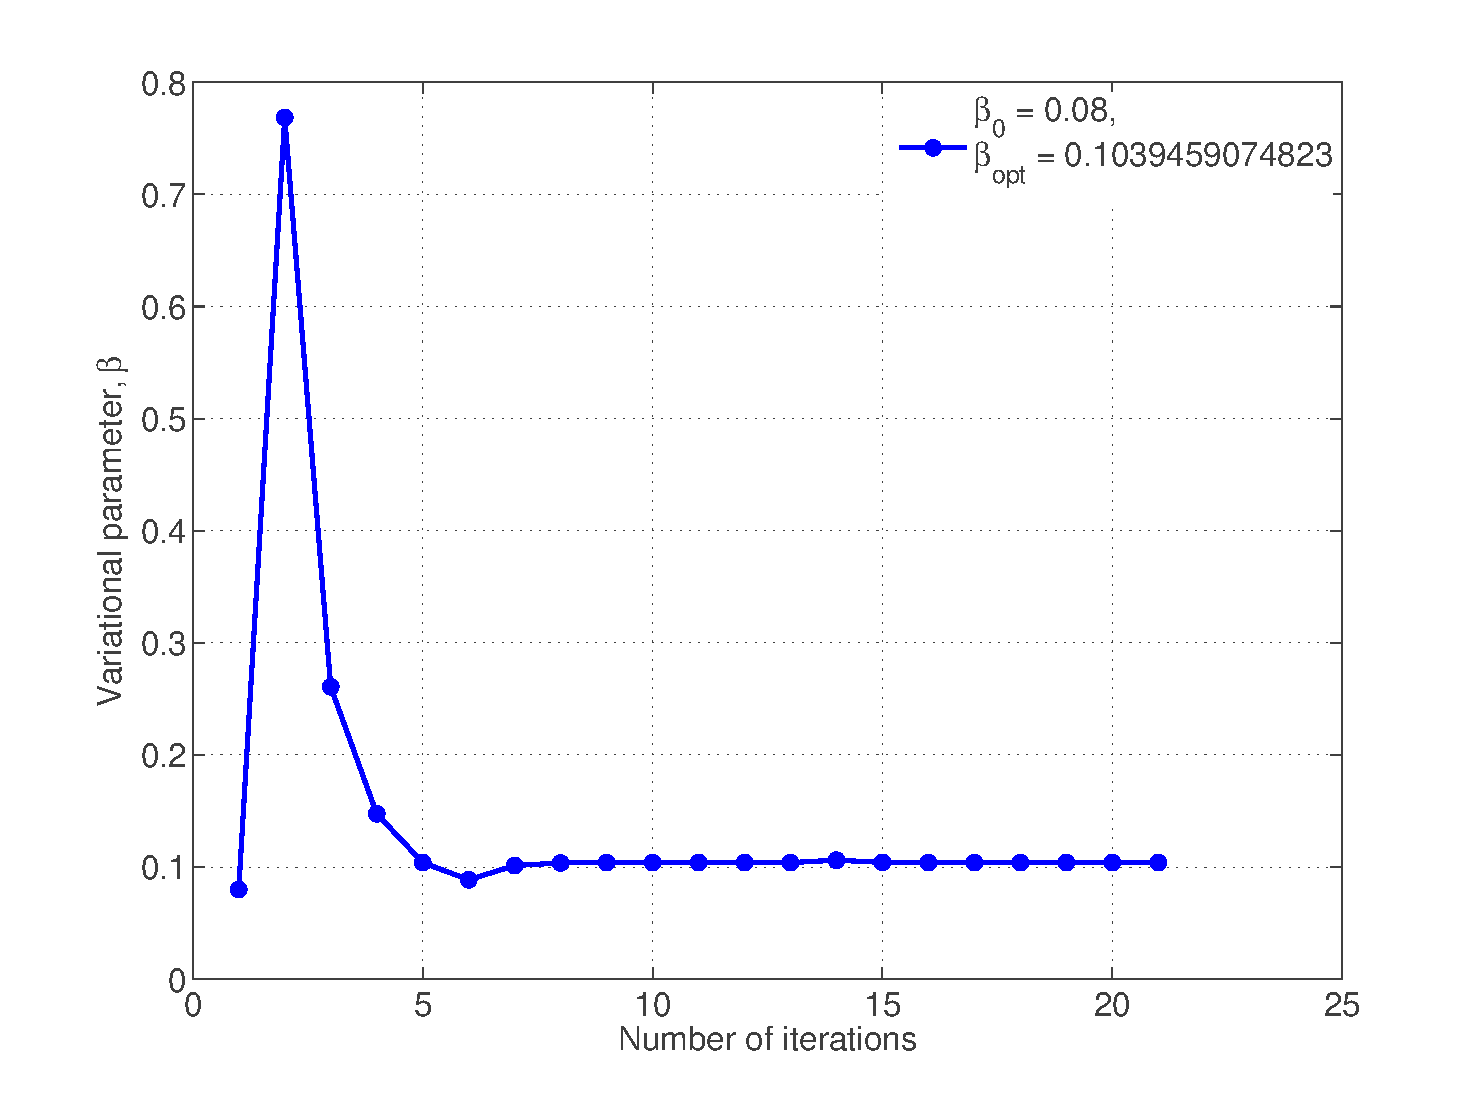
\includegraphics{figures/experimentalData/quasiNewtonOptimization/evolBetaBeOpt}}\\
    \end{tabular}
    \caption{Evolution of the variational parameters $\alpha$ and $\beta$ with the number of iterations during the optimization of the trial wave function of Be atom with the quasi-Newton method. The experiment was carried out with $10^7$ Monte Carlo cycles and $10 \%$ equilibration steps in four nodes.}
    \label{quasiNewtonOptBe}
  \end{center}
  \end{figure}
  \end{scriptsize}
\end{frame}




\begin{frame}{Convergence to the minimal energy for Be}
  \begin{scriptsize}
  \begin{figure}[!hbt]
  \begin{center}
    \resizebox{60mm}{!}{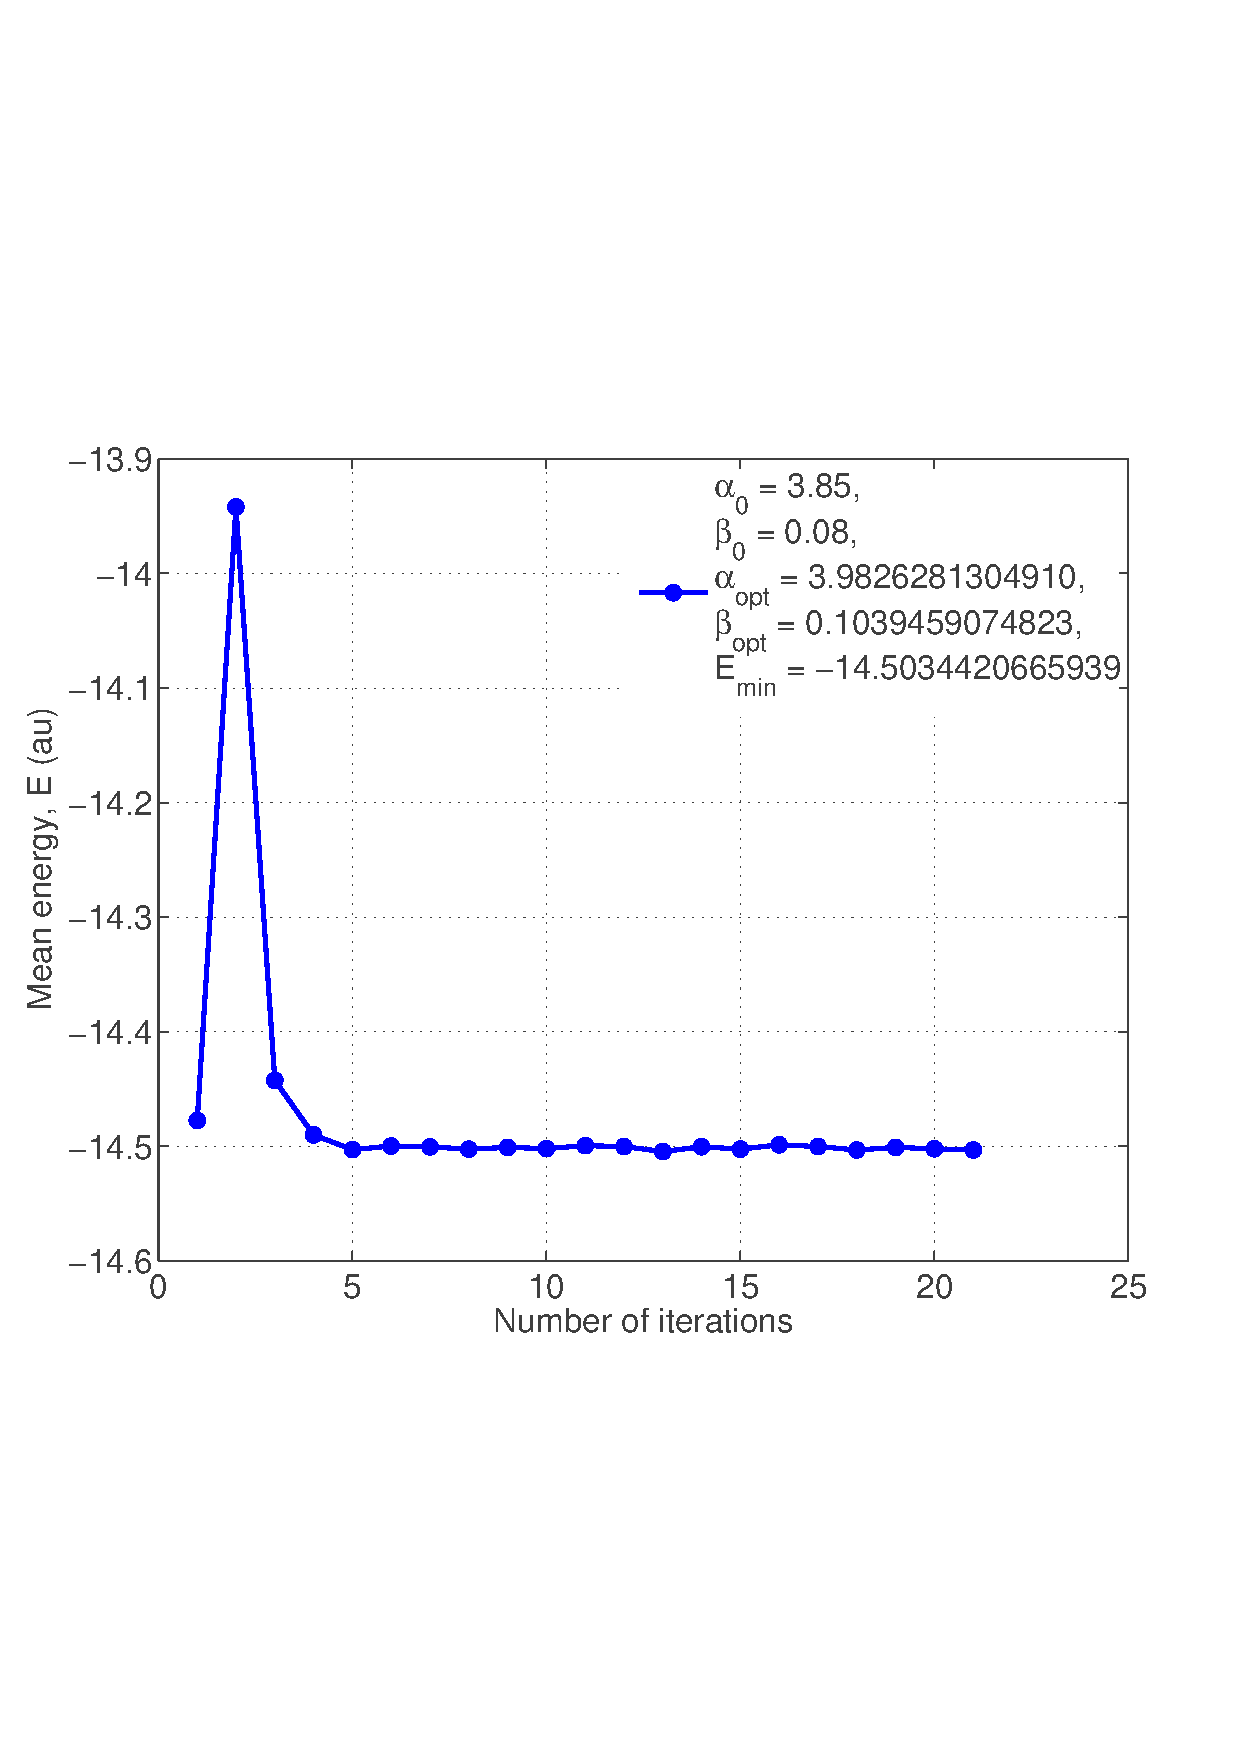
\includegraphics{figures/experimentalData/quasiNewtonOptimization/plotEnergyOptimizationBe}}\\
    \caption{Evolution of the energy with the number of iterations during the optimization of the trial wave function of Be atom with the quasi-Newton method. The experiment was carried out with $10^7$ Monte Carlo cycles and $10 \%$ equilibration steps in four nodes.}
    \label{quasiNewtonOptBe}
  \end{center}
  \end{figure}
  \end{scriptsize}
\end{frame}



%%%%%%%%%%%%%%% GROUND STATE ENERGIES %%%%%%%%%%%%%%%%%%%%%%
%%%%%%%%%%%%%%%%%%%%%%%%%%%%%%%%%%%%%%%%%%%%%%%%%%%%%%%%%%%%
\subsection{Extrapolation to zero dt}
\begin{frame}{Extrapolation of energy to zero dt for He}

  \begin{scriptsize}
  \begin{table}[!hbt]
  \centering
  \begin{tabular}{cccc}
    \toprule[1pt]
    \textbf{Time step} & \textbf{Energy}, (au)  & \textbf{Error} & \textbf{Accepted moves}, (\%) \\
    \midrule[1pt]
    0.002  & -2.891412637854  &  5.5e-4   &  99.97\\
    0.003  & -2.890797649433  &  4.5e-4   &  99.94\\
    0.004  & -2.890386198895  &  4.0e-4   &  99.91\\
    0.005  & -2.890078440930  &  3.5e-4   &  99.88\\
    0.006  & -2.890463490951  &  3.2e-4   &  99.84\\
    0.007  & -2.890100432462  &  2.8e-4   &  99.81\\
    0.008  & -2.889659923905  &  2.7e-4   &  99.77\\
    \bottomrule[1pt]
  \end{tabular}\caption{Energy computed for the He atom and the error associated as a function of the time step. Parameters: $10^7$ Monte Carlo cycles with 10 \% equilibration steps, $\alpha =  1.8379$ and $\beta = 0.3704$.}\label{blockingDtTableHe}
  \end{table}
  \end{scriptsize}
\end{frame}




\begin{frame}{Extrapolation of energy to zero dt for He}
  \begin{scriptsize}
  \begin{figure}[!hbt]
    \begin{center}
    \begin{tabular}{cc}
    \resizebox{50mm}{!}{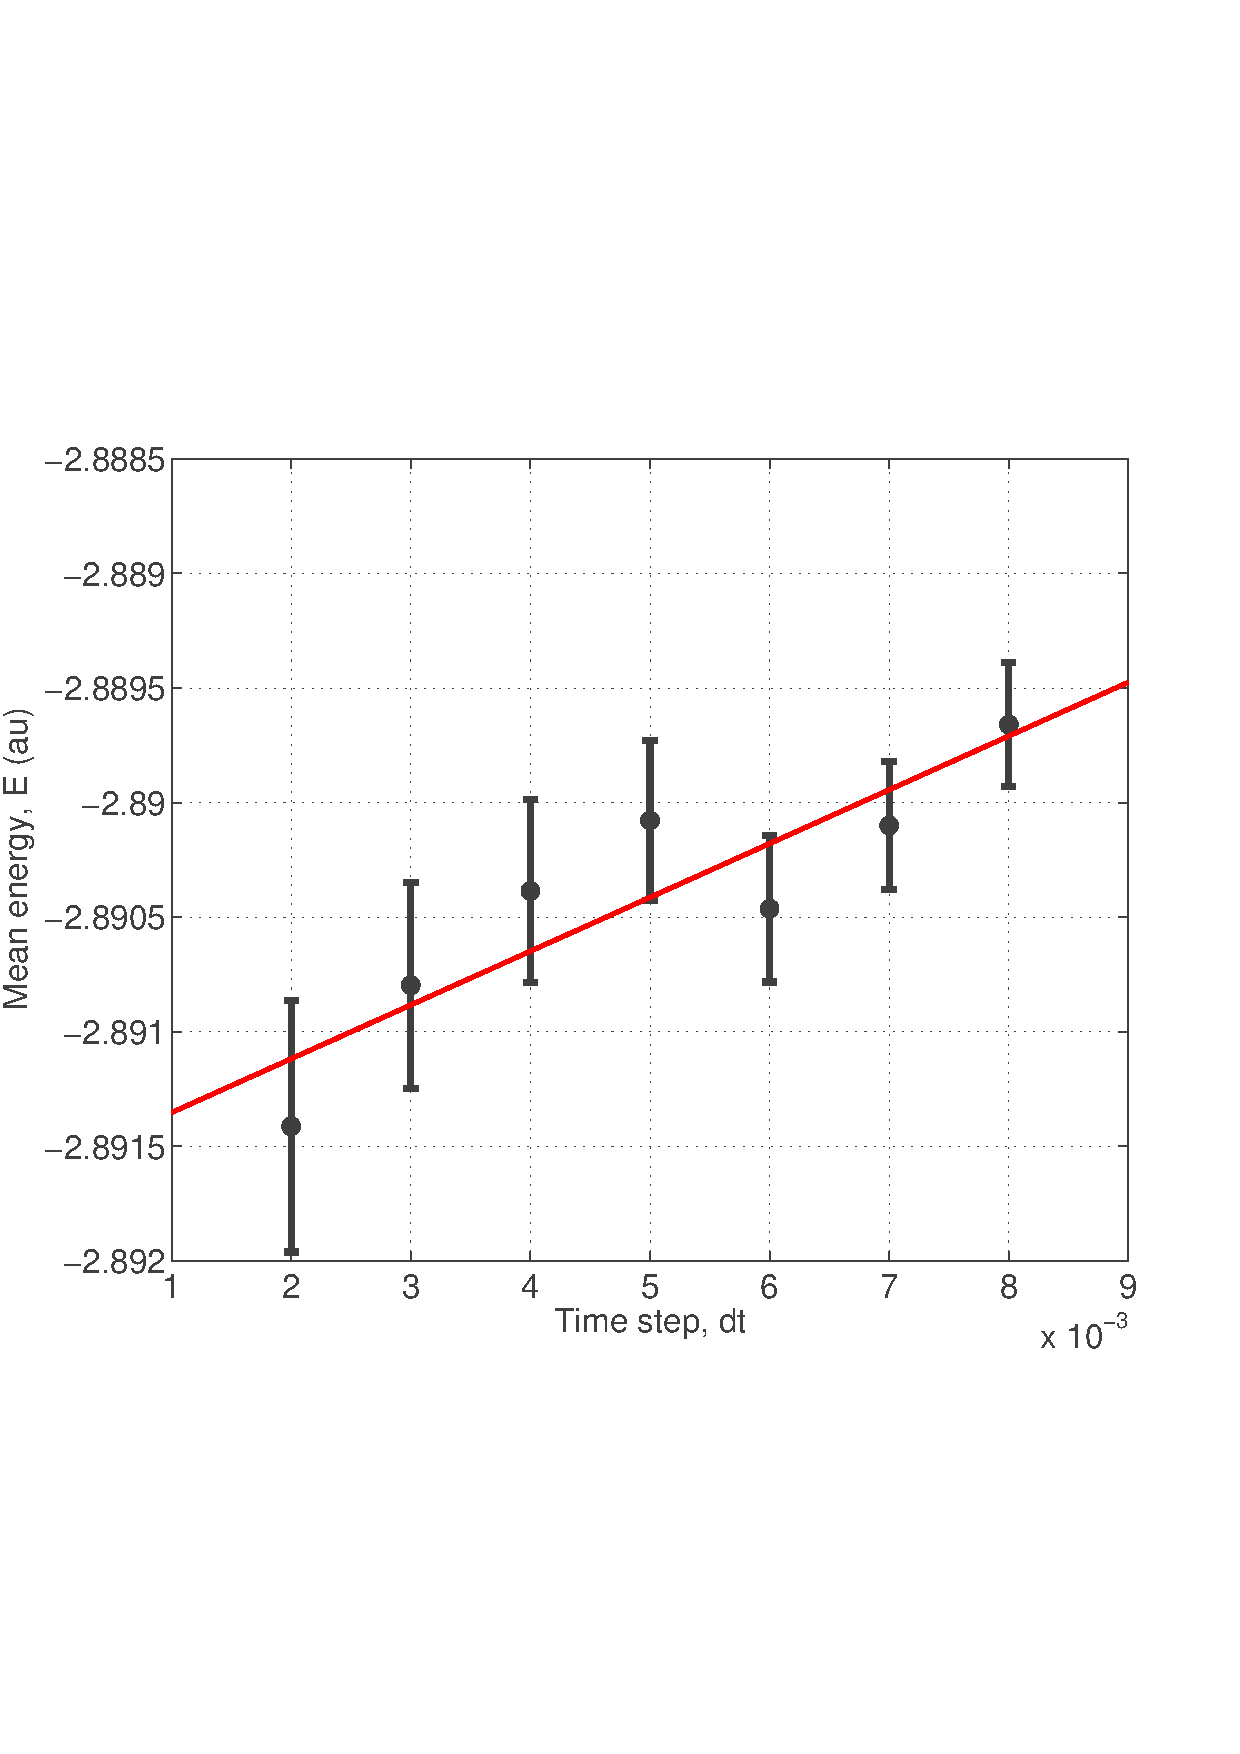
\includegraphics{figures/experimentalData/blocking/blockingDtHe}} &
      \resizebox{50mm}{!}{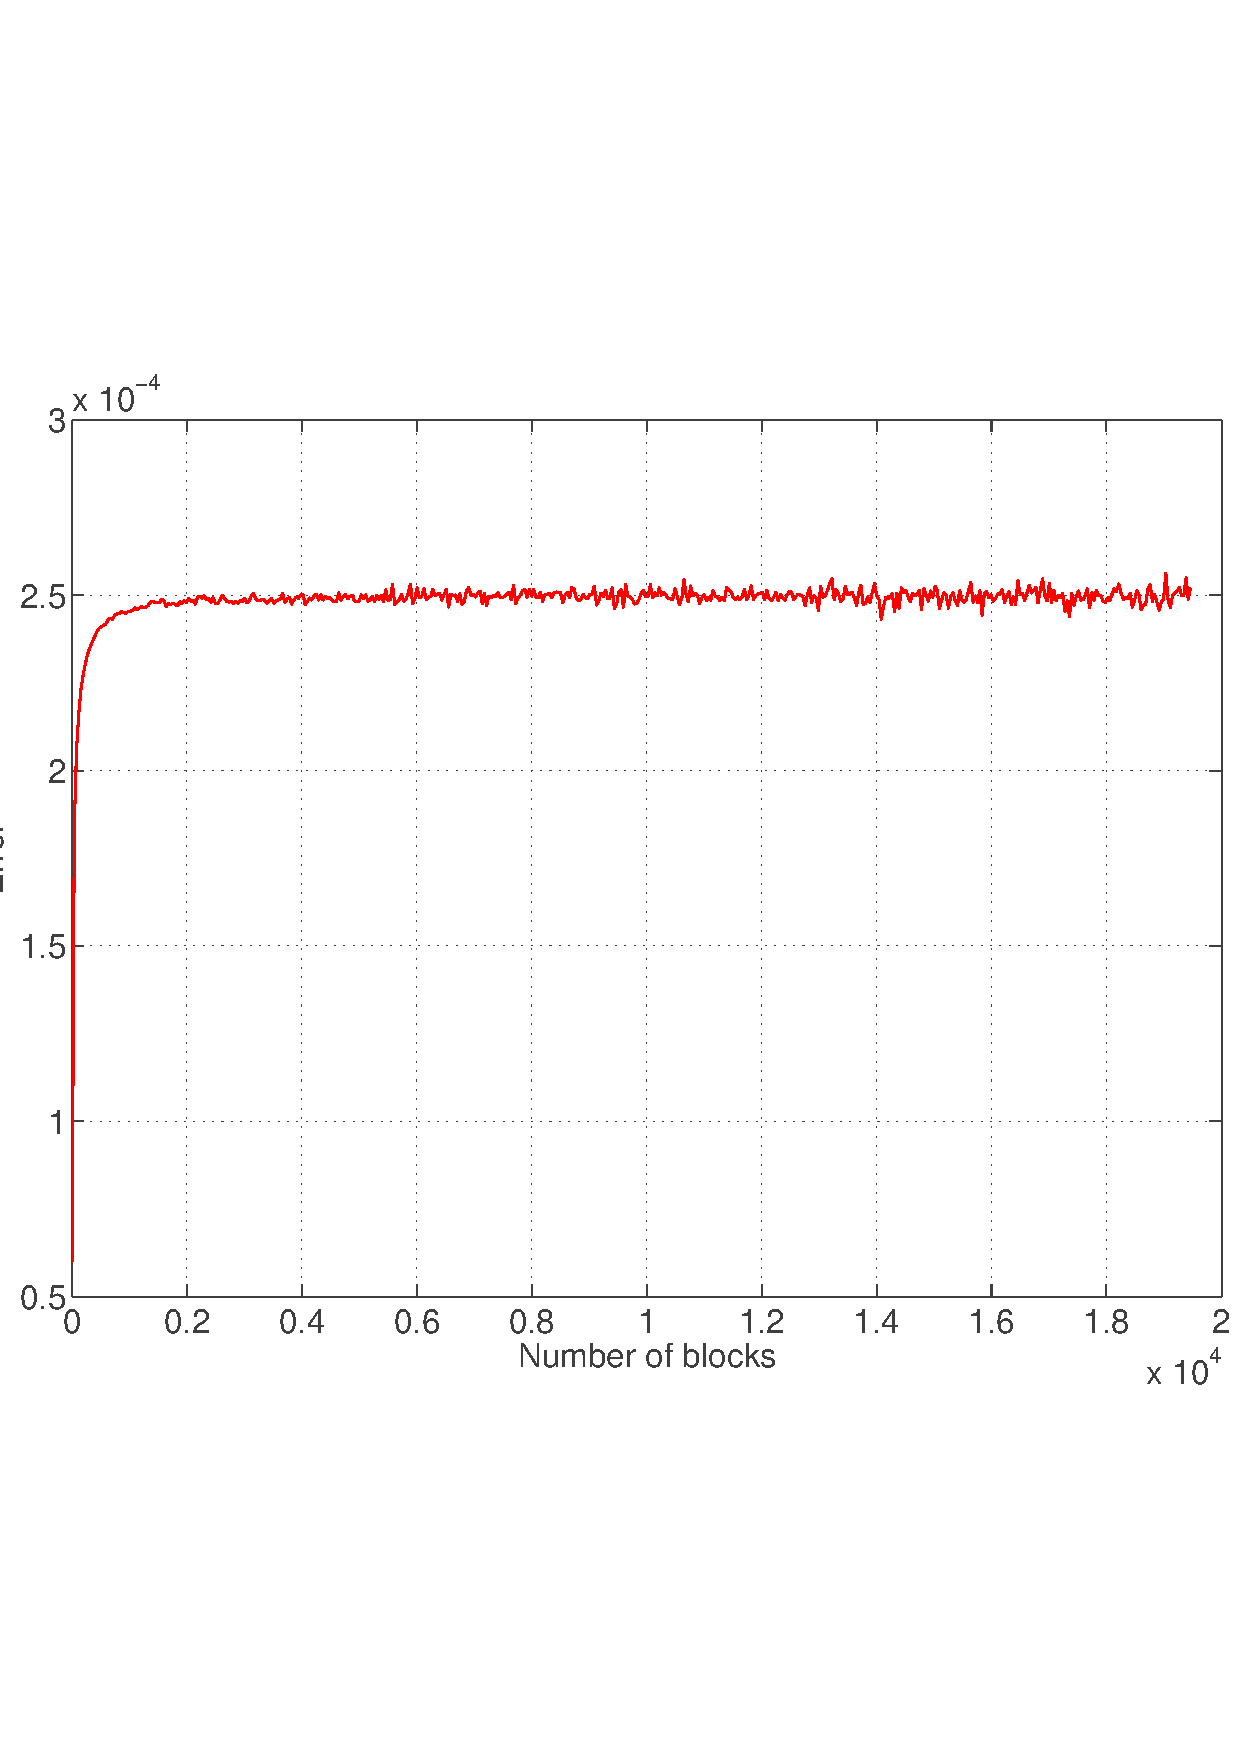
\includegraphics{figures/experimentalData/blocking/blockingHe}} \\
      \end{tabular}
      \caption{To the left we show the  extrapolation to $dt-$zero of the energy for a He atom. To the  right we display the details of the blocking analysis at $dt=0.01$ where the energy $-2.89039 \pm 2.5 \times 10^{-4}\, au$. Experimental setup: $10^7$ Monte Carlo cycles, $10 \%$ equilibration steps with four nodes, with $\alpha = 1.8379$, $\beta = 0.3704$.}
      \label{dtEnergyExtrapolationHe}
    \end{center}
  \end{figure}
  \end{scriptsize}  
\end{frame}




\begin{frame}{Extrapolation of energy to zero dt for Be}
  \begin{scriptsize}
  \begin{table}[!hbt]
  \centering
  \begin{tabular}{cccc}
    \toprule[1pt]
    \textbf{Time step} & \textbf{Energy}, (au)  & \textbf{Error} & \textbf{Accepted moves}, (\%) \\
    \midrule[1pt]
    0.004  &  -14.50321303316  &  1.3e-3  &   99.61\\
    0.005  &  -14.50266236227  &  1.2e-3  &   99.47\\
    0.006  &  -14.50136820967  &  1.1e-3  &   99.32\\
    0.007  &  -14.50314292468  &  1.0e-3  &   99.17\\
    0.008  &  -14.50206184582  &  9.5e-4  &   99.01\\
    0.009  &  -14.50164368104  &  8.5e-4  &   98.85\\
    0.01   &  -14.50145748870  &  8.0e-4  &   98.68\\
    \bottomrule[1pt]
  \end{tabular}\caption{Energy computed for the Be atom and the error associated as a function of the time step. Parameters: $10^7$ Monte Carlo cycles with 10 \% equilibration steps, $\alpha = 3.983$ and $\beta = 0.103$.}\label{blockingDtTableBe}
  \end{table}
  \end{scriptsize}
\end{frame}




\begin{frame}{Extrapolation of energy to zero dt for Be}
  \begin{scriptsize}
  \begin{figure}[!hbt]
    \begin{center}
      \begin{tabular}{cc}
      \resizebox{50mm}{!}{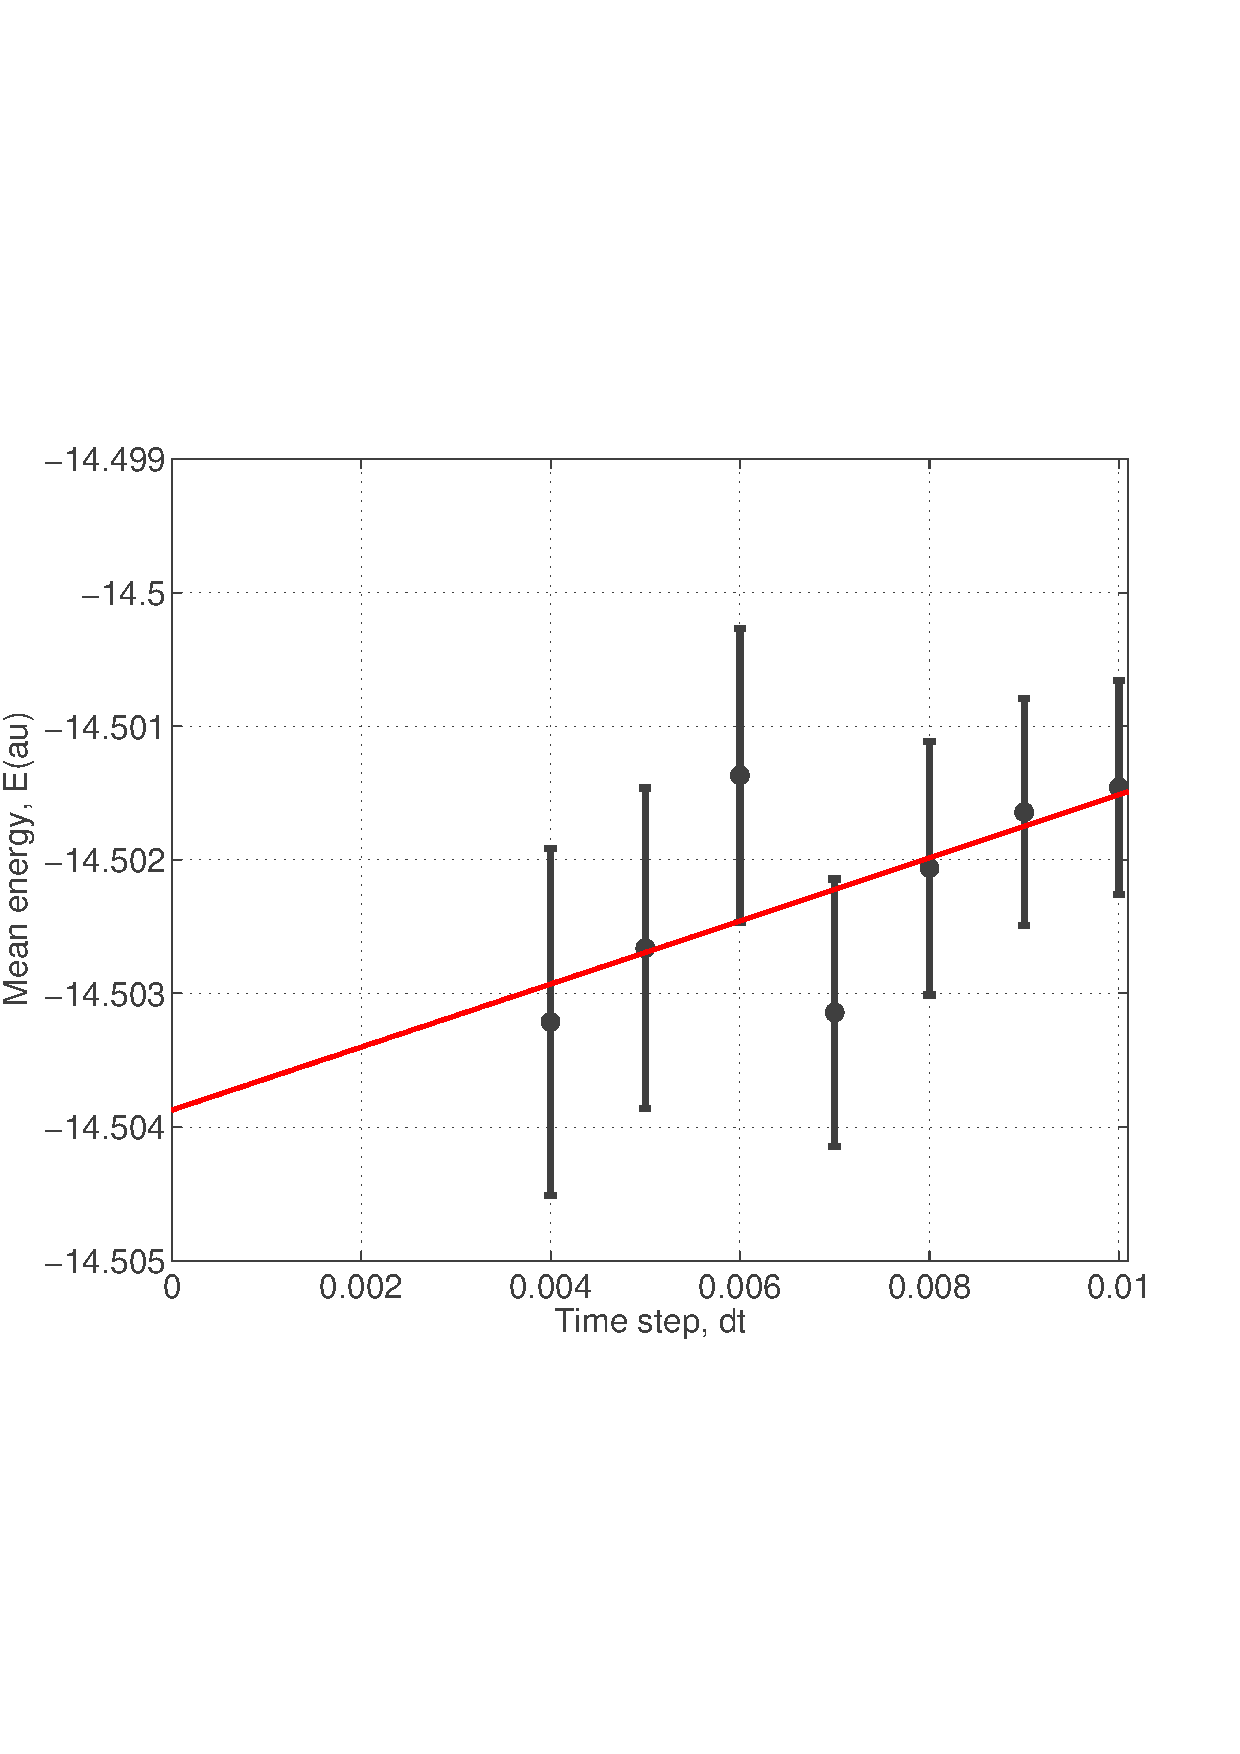
\includegraphics{figures/experimentalData/blocking/blockingDtBe}} &
      \resizebox{50mm}{!}{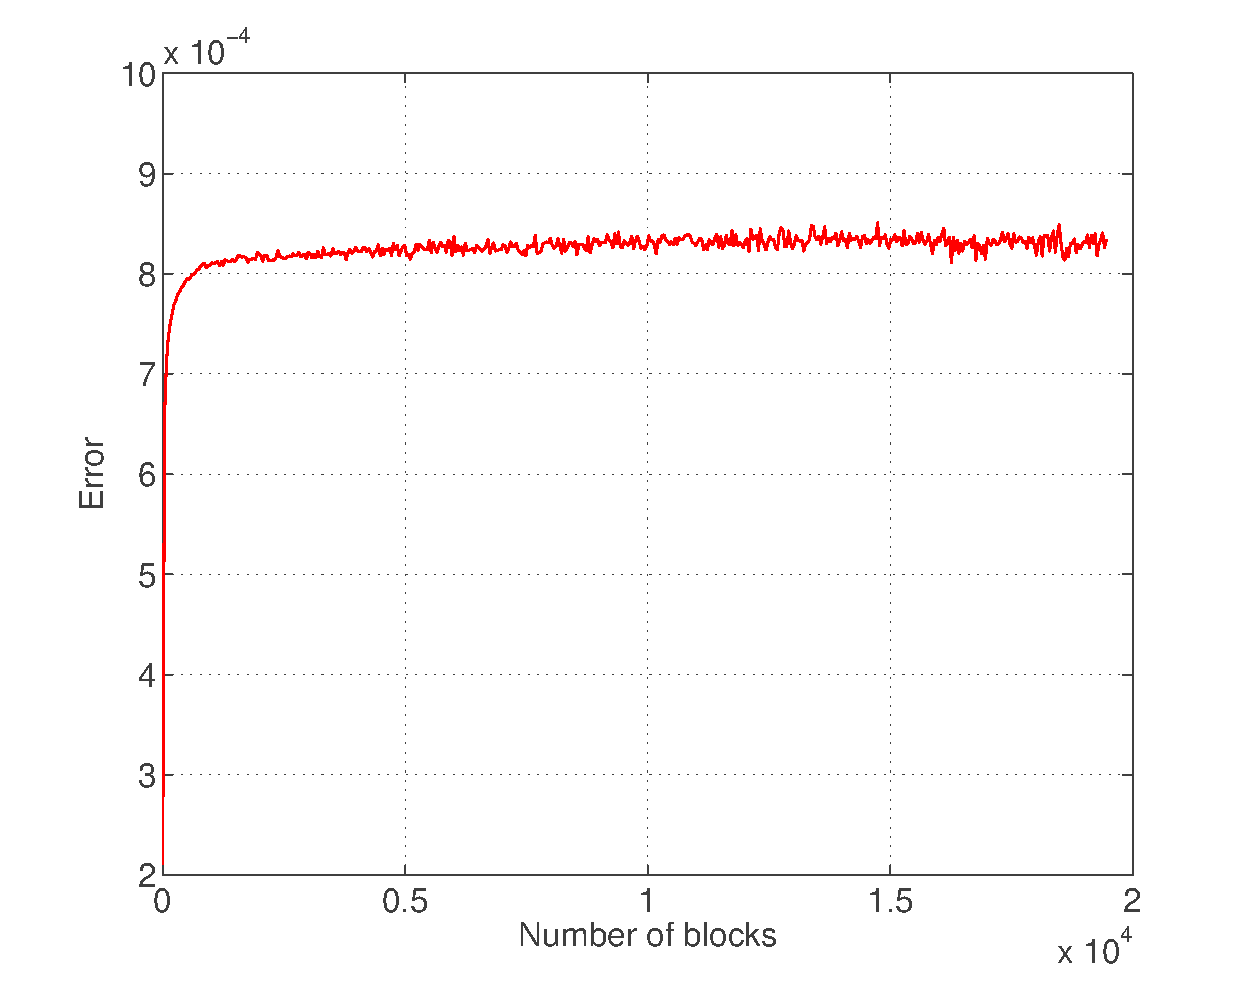
\includegraphics{figures/experimentalData/blocking/plotBlockingBe}} \\
      \end{tabular}
      \caption{Extrapolation to $dt-$zero of the energy (left) and blocking analysis at $dt=0.01$ for the Be atom where the energy $E = -14.50146 \pm 8.5 \times 10^{-4} \, au$. Experimental setup: $10^7$ Monte Carlo cycles, $10 \%$ equilibration steps for four nodes, with $\alpha = 3.983$ and $\beta = 0.103$.}
      \label{dtEnergyExtrapolationBe}
    \end{center}
  \end{figure}
  \end{scriptsize}
\end{frame}



\begin{frame}{Extrapolation of energy to zero dt for 2-$e^-$ electron QD}
  \begin{scriptsize}
  \begin{table}
  \centering
  \begin{tabular}{cccc}
  \toprule[1pt]
    \textbf{Time step} & \textbf{Energy}, (au)  & \textbf{Error} & \textbf{Accepted moves}, (\%) \\
    \midrule[1pt]
    0.01 & 3.000340072477 & 4.5e-5 & 99.95\\
    0.02 & 3.000357900850 & 3.2e-5 & 99.87\\
    0.03 & 3.000364180564 & 2.6e-5 & 99.77\\
    0.04 & 3.000384908560 & 2.2e-5 & 99.65\\
    0.05 & 3.000370330692 & 2.0e-5 & 99.52\\
    0.06 & 3.000380980039 & 1.8e-5 & 99.37\\
    0.07 & 3.000402836533 & 1.7e-5 & 99.21\\
    \bottomrule[1pt]
  \end{tabular}\caption{Results of a blocking analysis for several time steps. The system was a two-dimensional quantum dot with two electrons and $\omega=1.0$. The rest of the parameters were: $10^7$ Monte Carlo cycles with 10 \% equilibration steps, and $\alpha = 0.99044$ and $\beta = 0.39994$ taken from  Albrigtsen(2009).}\label{blockingDtTable2DQDot2e}
  \end{table}
  \end{scriptsize}
\end{frame}




\begin{frame}{Extrapolation of energy to zero dt for 2-$e^-$ electron QD}
  \begin{scriptsize}
  \begin{figure}[!hbt]
    \begin{center}
      \begin{tabular}{cc}
      \resizebox{50mm}{!}{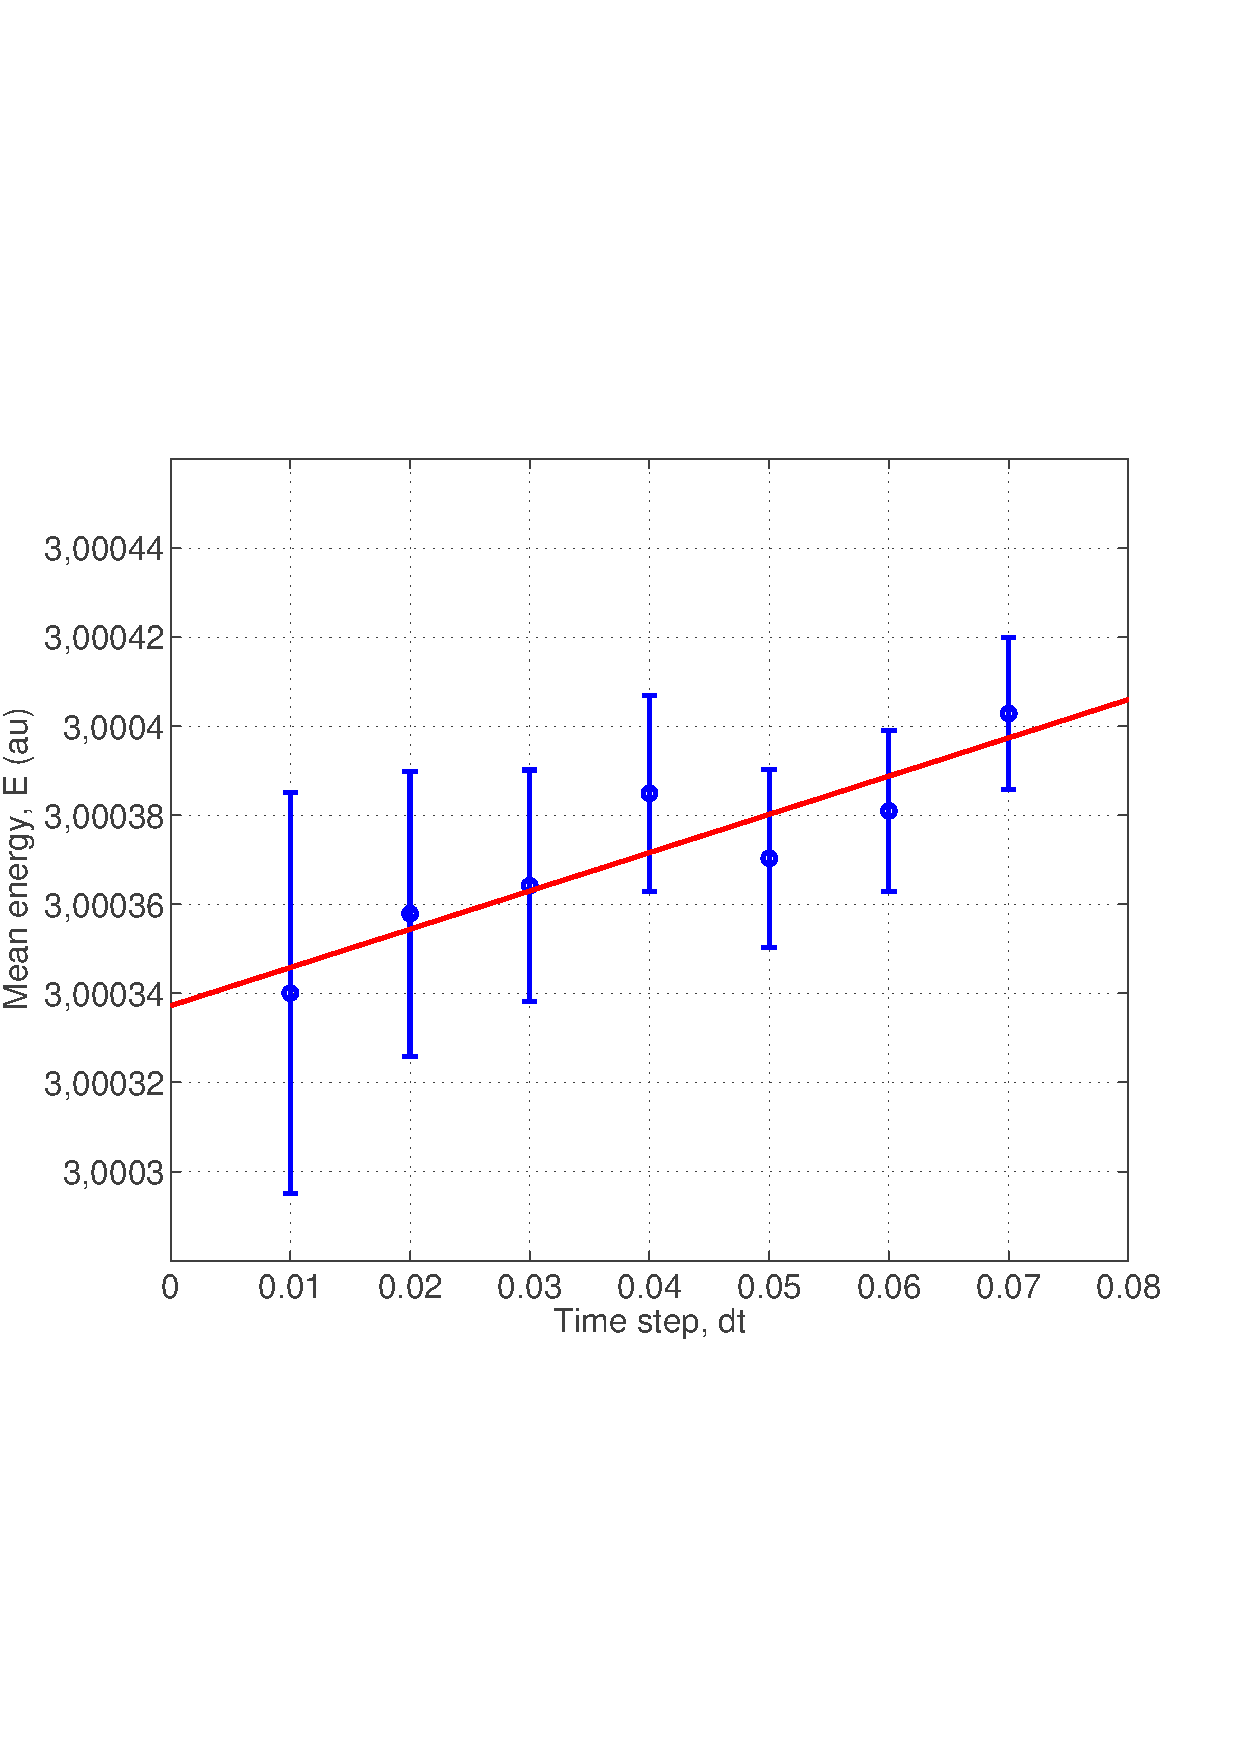
\includegraphics{figures/experimentalData/blocking/dtPlot2DQDot2e}} &
      \resizebox{50mm}{!}{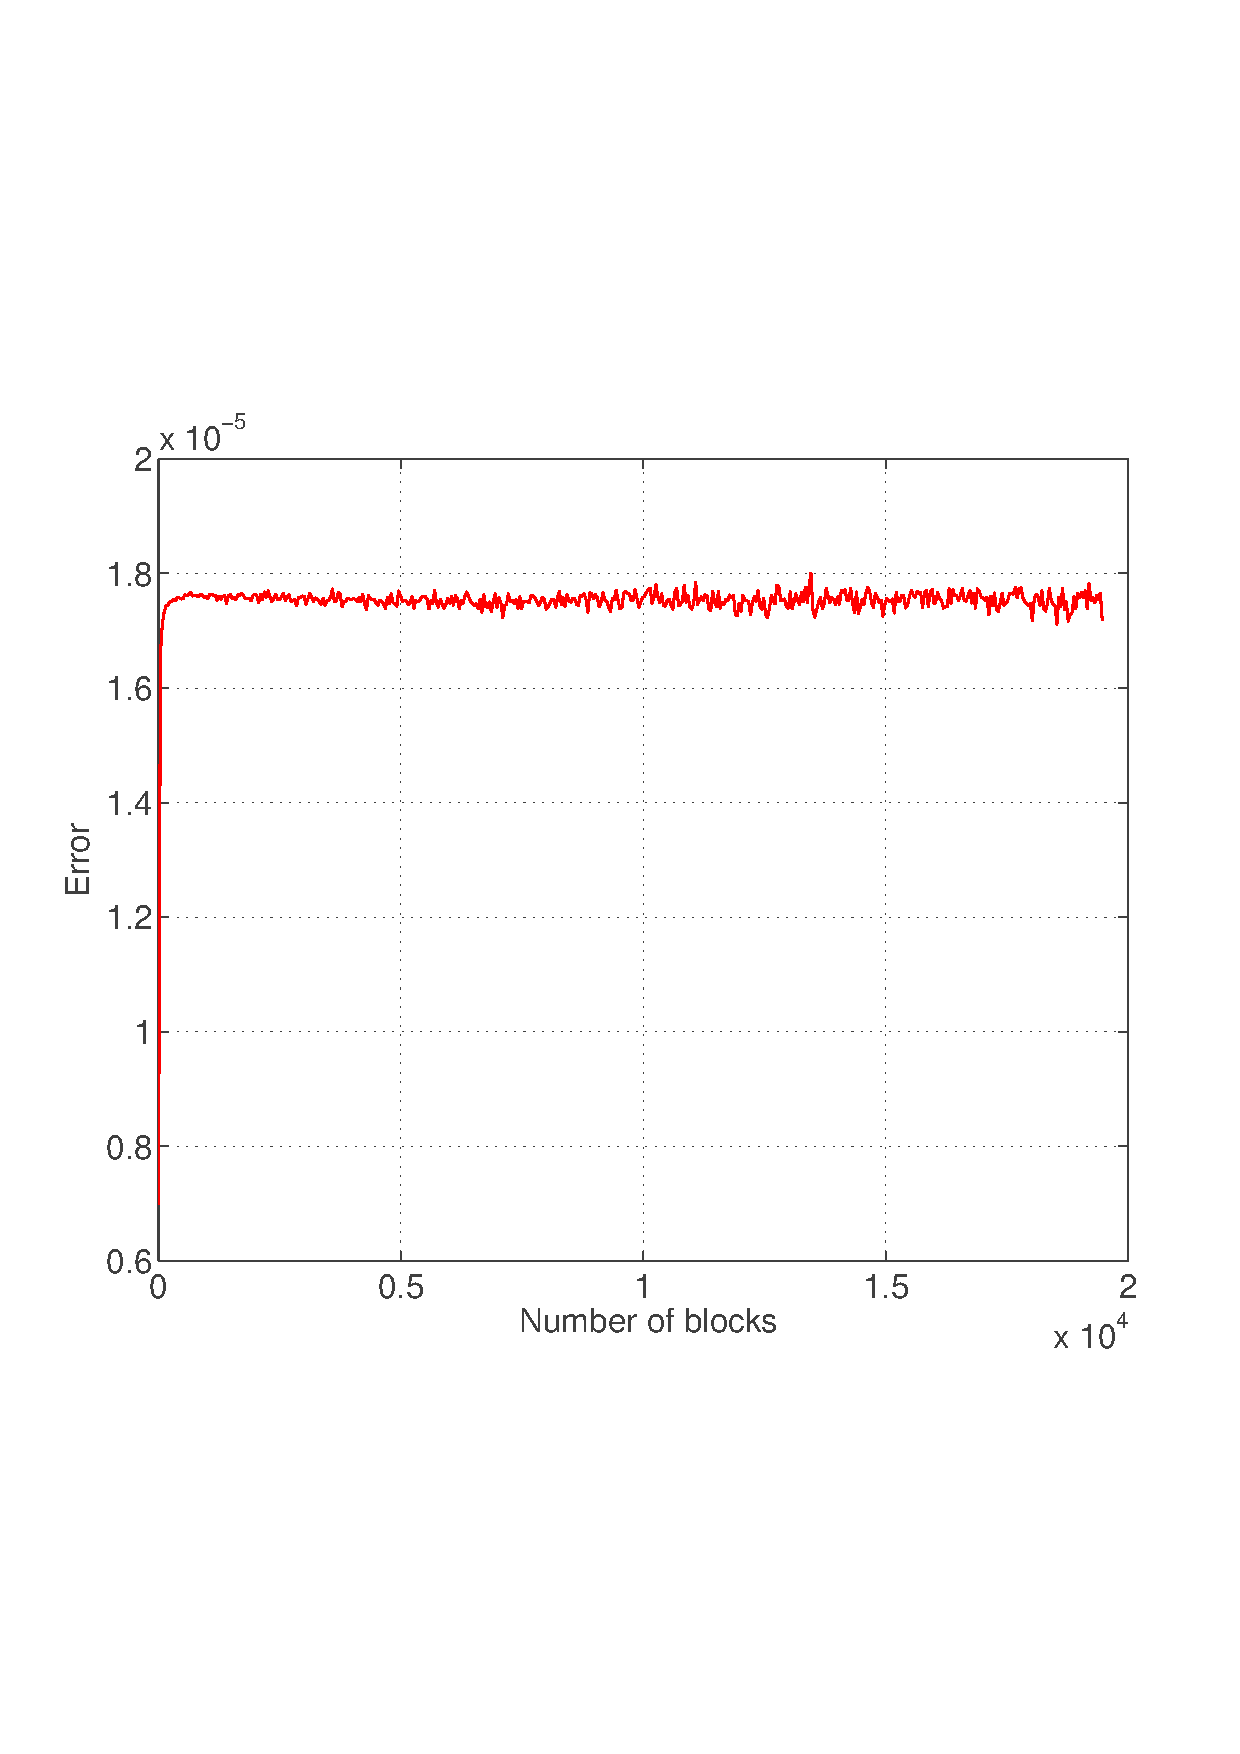
\includegraphics{figures/experimentalData/blocking/block2DQDot2edt0p06}} \\
      \end{tabular}
      \caption{Extrapolation to $dt-$zero of the energy for a two-dimensional quantum dot with two electrons (left) and mean energy error ($E_{min} = 3.000381 \pm 1.8 \times 10^{-5} \, au$) at $dt=0.06$ as a function of the number of blocks for a 2DQDot2e (right). Parameters of simulation: $1 \times 10^7$ Monte Carlo steps with 10 \% equilibration steps, $\alpha = 0.99044$ and $\beta = 0.39994$. The error varies from $1.7 \times 10^{-5}$ at $dt = 0.07$ to $4.5\times 10^{-5}$ at $dt = 0.01$.}
      \label{dtEnergyExtrapolation2DQdot2e}
   \end{center}
  \end{figure}
  \end{scriptsize}
\end{frame}



\begin{frame}{Extrapolation of energy to zero dt for 6-$e^-$ electron QD}
  \begin{scriptsize}
  \begin{table}
  \centering
  \begin{tabular}{cccc}
    \toprule[1pt]
    \textbf{Time step} & \textbf{Energy}, (au)  & \textbf{Error} & \textbf{Accepted moves}, (\%) \\
    \midrule[1pt]
    0.01 & 20.19048030567 & 4.0e-4 & 99.90\\
    0.02 & 20.19059799459 & 2.8e-4 & 99.75\\
    0.03 & 20.19045049792 & 2.4e-4 & 99.55\\
    0.04 & 20.19069748408 & 2.0e-4 & 99.34\\
    0.05 & 20.19066469178 & 1.8e-4 & 99.10\\
    0.06 & 20.19064491561 & 1.7e-4 & 98.85\\
    0.07 & 20.19078449010 & 1.6e-4 & 98.58\\
    \bottomrule[1pt]
  \end{tabular}\caption{Results of a blocking analysis for several time steps. The system was a two-dimensional quantum dot with six electrons and $\omega=1.0$. The rest of the parameters were: $10^7$ Monte Carlo cycles with 10 \% equilibration steps, and $\alpha = 0.926273$ and $\beta = 0.561221$ taken from Albrigtsen (2009).}\label{blockingDtTable2DQDot6e}
  \end{table}
  \end{scriptsize}
\end{frame}




\begin{frame}{Extrapolation of energy to zero dt for 6-$e^-$ electron QD}
  \begin{scriptsize}
  \begin{figure}[!hbt]
    \begin{center}
      \begin{tabular}{cc}
      \resizebox{50mm}{!}{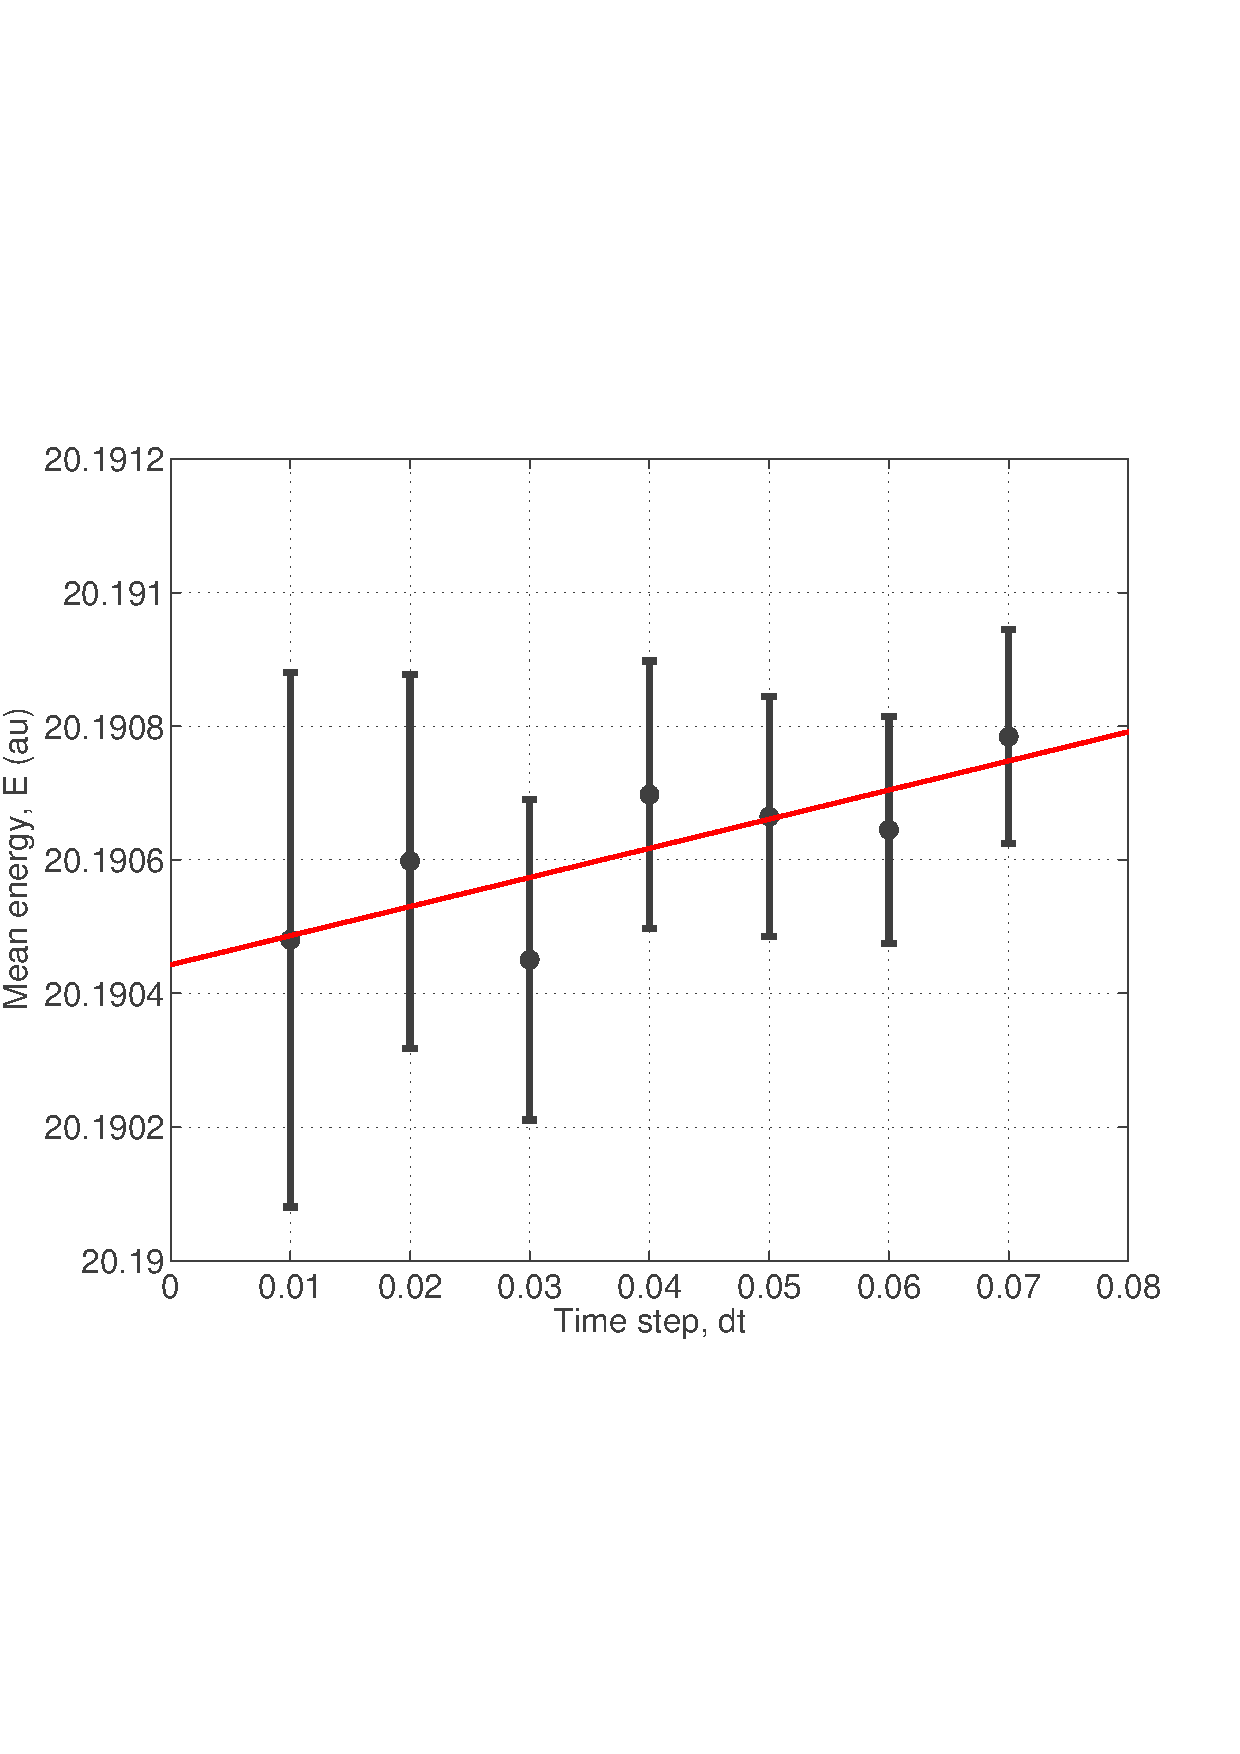
\includegraphics{figures/experimentalData/blocking/plotDtStudy2DQDot6e}} &
      \resizebox{50mm}{!}{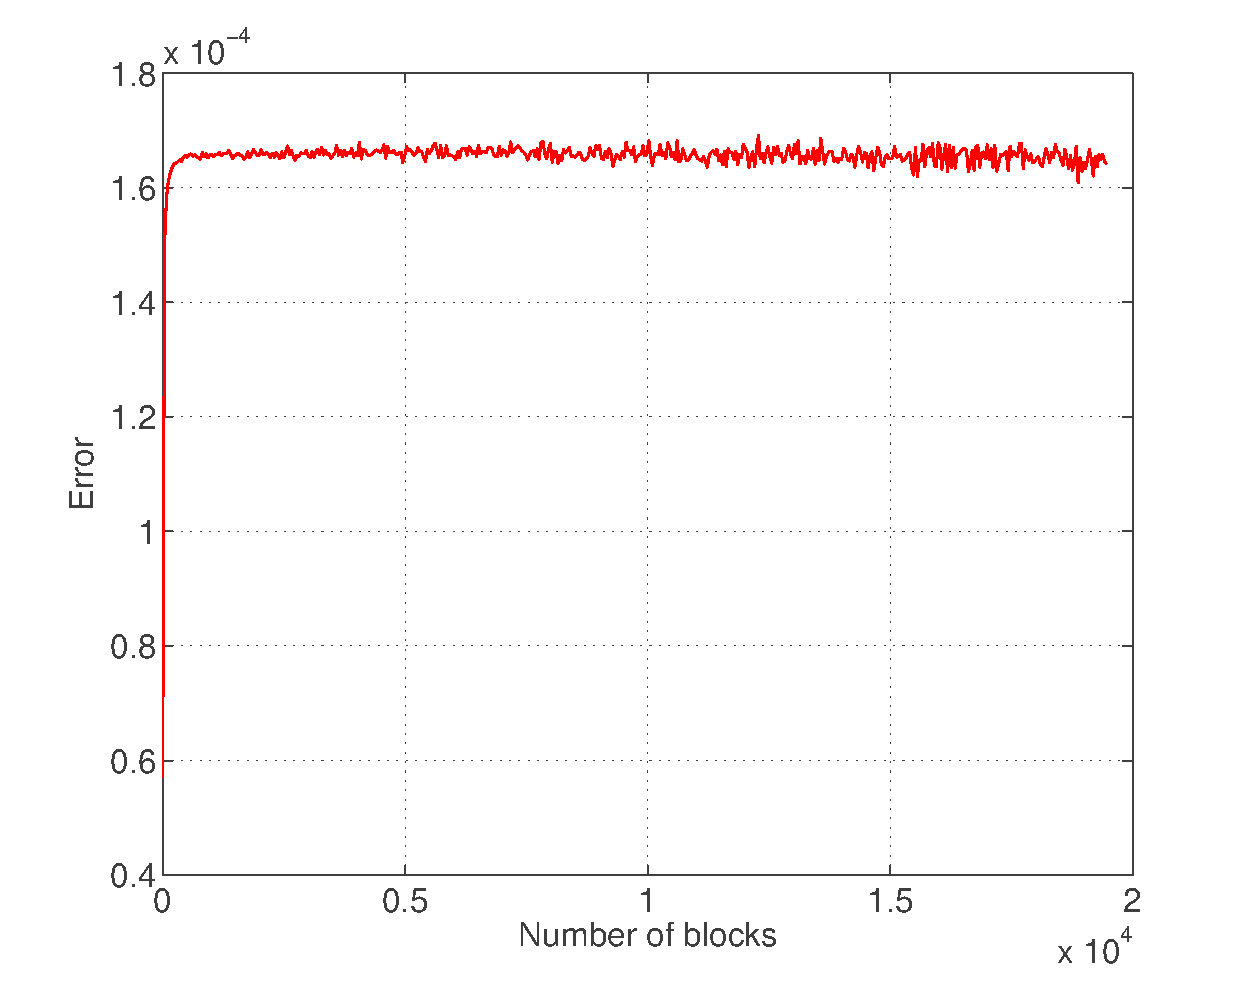
\includegraphics{figures/experimentalData/blocking/blockAnalyse2DQDot6e}}\\
      \end{tabular}
      \caption{Extrapolation to $dt-$zero of the energy for a two-dimensional quantum dot with six electrons (left) and mean energy error ($E_{min} = 20.190645 \pm 1.7 \times 10^{-4} \, au$) at $dt=0.06$ as a function of the number of blocks for a 2DQDot6e (right). Parameters of simulation: $10^7$ Monte Carlo steps with 10 \% equilibration steps, $\alpha = 0.926273$ and $\beta = 0.561221$ running with four nodes.}
      \label{dtEnergyExtrapolation2DQdot6e}
    \end{center}
  \end{figure}
  \end{scriptsize}
\end{frame}




\begin{frame}{Extrapolated energy to zero dt for atoms and QD}
  \begin{scriptsize}
  \begin{table}
  \centering
  \begin{tabular}{lr}
    \toprule[1pt]
    \textbf{System} & \textbf{Energy}, (au)\\
    \midrule[1pt]
    He &  -2.8913\\
    Be &  -14.5039\\
    2DQDot2e & 3.0003\\
    2DQDot6e & 20.1904\\
    \bottomrule[1pt]
  \end{tabular}\caption{Energies estimated using zero-dt extrapolation.%$\omega~=~1.0$ for quantum dots.
  }\label{energyCuts}
  \end{table}
  \end{scriptsize}
\end{frame}



\subsection{Influence of the \# MC cycles}
\begin{frame}{Influence of the \# MC cycles on the statistical error}
  \begin{scriptsize}
  \begin{figure}[!hbt]
    \begin{center}
%        \begin{tabular}{cc}
      \resizebox{55mm}{!}{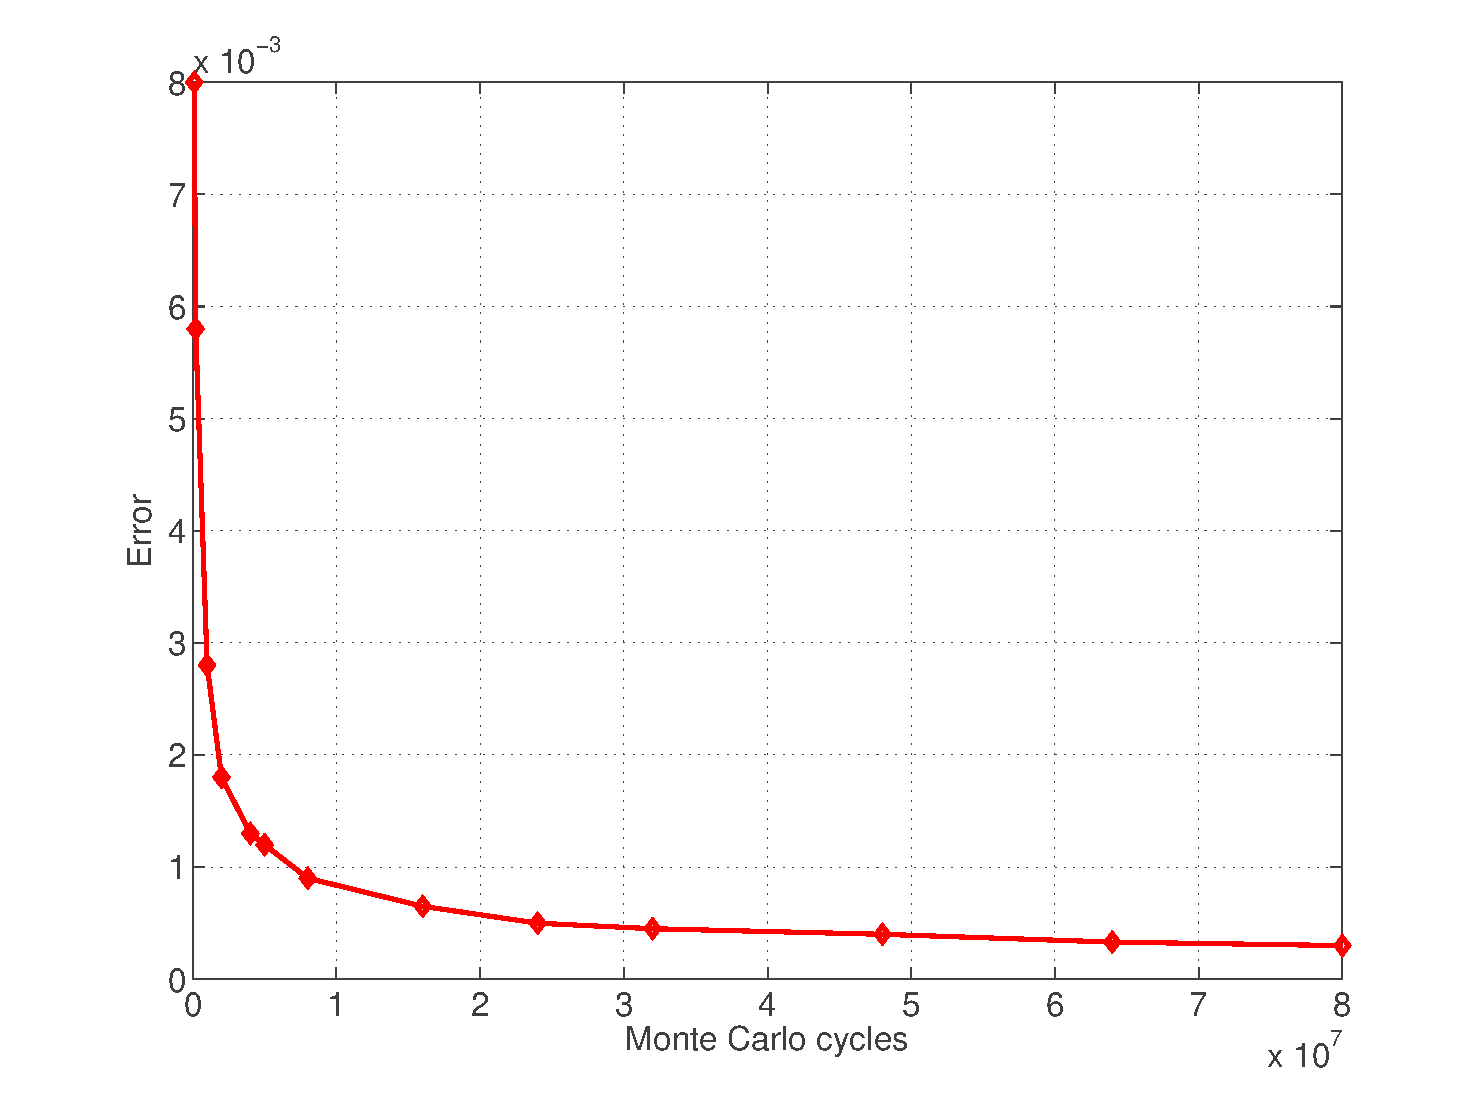
\includegraphics{figures/experimentalData/errorVsMC/errorVsMonteCarloBe}}
%       \resizebox{55mm}{!}{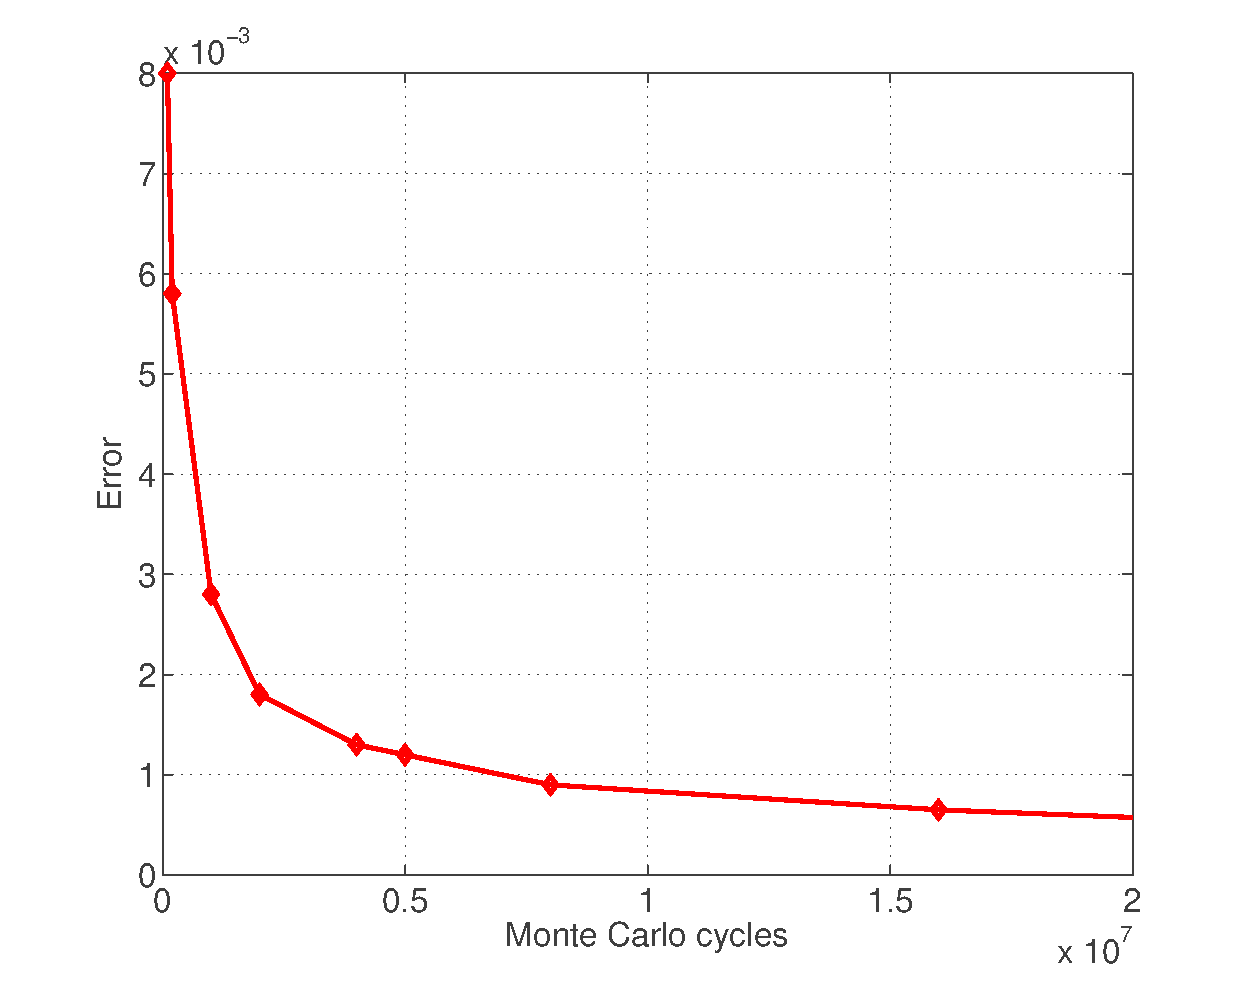
\includegraphics{figures/experimentalData/errorVsMC/errorVsMonteCarloBeZoom}}\\
%        \end{tabular}
      \caption{Error in the energy obtained by blocking for a Be atom as a function of the number of Monte Carlo cycles. The set up for the experiment was: $dt = 0.01$, $\alpha = 3.981$, $\beta = 0.09271$, 10 \% equilibration steps by run in parallel with four processors.}
      \label{errorVsMcBe}
    \end{center}
  \end{figure}
  \end{scriptsize}
\end{frame}










